\documentclass[11pt]{report}
\renewcommand{\baselinestretch}{1.1}
\usepackage[utf8]{inputenc}
\usepackage{amsmath,mathtools}
\usepackage{tcolorbox}
\usepackage{multirow}
\newcommand{\mbf}[1]{\mathbf{#1}}
\newcommand{\tbf}[1]{\textbf{#1}}
\newcommand{\dsum}[3]{$\sum^{#1}_{#2}{#3}$}
\newcommand{\dint}[3]{\int^{#1}_{#2}{#3}}
\newcommand{\tit}[1]{\textit{#1}}
\newcommand{\fn}[1]{\footnote{#1}}
\newcommand{\de}[2]{\frac{d{#1}}{d{#2}}}
\newcommand{\ch}[2]{\Gamma^{#1}_{#2}}
\newcommand{\chris}{\ch{\mu}{\alpha \beta}=\frac{1}{2}g^{\mu \lambda}(\p_{\alpha} g_{\beta \lambda}+\p_\beta g_{\alpha \lambda} - \p_\lambda g_{\alpha \beta})}
\newcommand{\p}{\partial}
\newcommand{\pe}[2]{\frac{\partial{#1}}{\partial{#2}}}
\newcommand{\n}{\nonumber}
\newcommand{\cbox}{tcolorbox}
\newcommand{\cc}[1]{\left({#1}\right)}
\newcommand{\rr}[1]{\left[{#1}\right]}
\newcommand{\vd}[1]{\dot{\vec{#1}}}
\newcommand{\tx}[1]{\text{#1}}

\begin{document}
\title{Cluster Mergers}
\author{Divesh Jain}
\maketitle
\tableofcontents

\chapter{Introduction}
The idea of this document is to basically cover all theoretical aspects of areas and bootstrapping related to Ruta's project. 
\begin{itemize}
\item Understanding theory behind radiation
\item cover synchrotron and review papers eventually
\item How shocks lead to Cosmic Rays(finding a connection between radio and X-ray) - \textbf{Read VanWeeren Review}
\item The type of mechanism involved in particle acceleration(Fermi I and Fermi II Order acceleration ) - \textbf{Read Brunetti Review}
\end{itemize}
Over many areas, one area I am thoroughly interested is in particle acceleration mechanism.
\chapter{Basics behind Radiation}
\section{Principles of Special Relativity}
To describe a physical process we require both spatial and temporal co-ordinates of the events, which can be put to a single entity of four numbers $x^i=(t,\mbf{x})$. For the purpose of this article and following sections to come Latin indices \tit{a,b,c..,i,j,k} run over 0 , 1, 2 and 3; where 1, 2, 3 denote space dimensions.The Greek indices would be used to represent just the spatial dimensions.\\

In the following discussion we pay special attention to a subset of coordinate systems, called \textbf{inertial coordinate systems.} \\
\textbf{How do we create this inertial coordinate system?}\\
These coordinates systems, are defined by the property that a material particle, far removed from all external influences, will move with uniform velocities in such systems. verify this criterion. \textbf{But, there is no fundamental reason why any one class of coordinate systems should be preferred over others except for mathematical convenience.}Just to make our lives simpler, we still postulate that such a set of coordinates exists where any frame moves with uniform velocity with respect to an inertial frame.\\

\textbf{Rules of the game}
It is experimentally found that these two statements are true:
\begin{itemize}
\item All laws of nature are identical in all frames of reference, that is, the equations expressing the laws of nature are invariant in form with respect to the coordinate transformation connecting two frames.
\item Interactions between material particles does not take instantaneously and there exists a maximum speed of propagation for information of interaction. We call it \tit{c}.
\end{itemize}

The implication of the first point here is, that \tbf{the maximum speed of information propagation is same in all inertial frames.}



Section copied from paddy's book:\\
\textbf{To begin with, this result rules out any absolute nature for simultaneity; two events that appear to occur at the same time in one inertial frame will not, in general, appear to occur at the same time in another inertial frame.}\\
\textbf{Another important consequence requires first a mathematical construct. We define
\begin{equation}
ds^2=c^2dt^2 - dx^2 - dy^2 - dz^2
\end{equation}
If $ds=0$ in one frame then it implies that infinitesimally separated events $\mbf{P\text{ and } Q}$ with coordinates $x^i$ and $x^i+dx^i$ can be connected by a light signal. And because speed of light is same in all inertial frames, therefore $ds^\prime=0$ is also true in other frame of references. }
\\
\textbf{We want to find the value of this length element in different inertial frames, to do that}:\\
As a second step what we do is to treat $ds^2$ as a function of $(ds^\prime)^2$ and we can expand $ds^2$ as a function of $(ds^\prime)$ given as
\begin{eqnarray*}
ds^2=\alpha + a ds^{\prime^2}\\
\text{Now for $ds=0$, the distance element  $ds^\prime=0$ } \implies \alpha=0\\
\end{eqnarray*}  
We propose, that $a$ be a function of relative velocity $V$ between frames. Further, homogeneity and isotropy would require that $a(\mbf{V})$ be only a function of magnitude of $|\mbf{V}|$.
\section{Basics Of Electromagnetic Radiation}
\subsection{External Fields Of Force}

\subsection{Introduction to radiation from an accelerated charge}
The Electric Field in case of a stationary charged particle or charge moving with constant velocity falls as $r^{-2}$. When the charged particle accelerates then, the charge picks up a part which falls as $r^{-1}$, called the \textbf{radiation field}.\\
A field which falls as $E \propto r^{-1}$, has an energy flux $S \propto E^2 \propto r^{-2}$; we also know that the surface area of sphere increases as $r^2$. \textbf{Therefore in case of an accelerating charge, same amount of energy will flow through spheres of different radii, and also allows radiation field to travel large distances.}
\\
\subsubsection{Understanding Why accelerated charge radiate?}
\textbf{What is the $r$ dependence in Electric Field? }\\
From an earlier equation $\mbf{A}$ scales as the velocity $\mbf{v}$ of the charge. Because $\dot{\mbf{A}}$ contributes to E, there will be one  term in $\mbf{E}$ that is $\propto \; \; \mbf{a}$. This is, of course, in addition to the usual coulomb term that is independent of $\mbf{a}$ and falls as $\mbf{r}^{-2}$. As electric field is linear in charge $q$ as well,this term is linear in $q$. \\

Let us consider this electric field in the instantaneous rest frame, then a general form 
\begin{equation}
E=C(\theta)\frac{qa}{c^nr^m}=C(\theta) \cc{\frac{q}{r^2}}\cc{\frac{a}{c^nr^{m-2}}}
\end{equation}
C is dimensionless which depends $\theta$ between $\mbf{r \text{ and } a}$ and n and m need to be determined.(Because $v=0$ in the instantaneous rest  frame, the field cannot depend on the velocity). By dimensional analysis, it immediately follows that n=2 and m=1 . Hence
\begin{equation}
E=C\frac{qa}{c^2r}
\end{equation}
Hence we have a $r^{-1}$ dependence.
For C($\theta$)
\section{Radiation by Moving Charges}
Before we start with the chapter, we accept the fact that \textbf{accelerated charges emits electromagnetic radiation.}For, non relativistic motion the radiation is well described by Larmor's result.\\
We, first define Lienard-Wiechart Potentials and try to describe Fields for a Point Charge.
\subsection{Lienard-Wiechart Potentials for a point charge}
If there are no \textbf{Incoming Fields}, then the 4-vector potential caused by a charged particle in motion is:
\begin{equation}\label{Vpot}
A^\alpha(x)=\frac{4 \pi}{c}\int d^4x^\prime D_r(x-x^\prime)J^\alpha(x^\prime)
\end{equation}
where $D_r(x-x^\prime)$ is the \textbf{retarded Green Function} and 4-vector current is given as:
\begin{equation}\label{Cden}
J^\alpha(x^\prime)=ec\int d\tau V^\alpha(\tau)\delta^{(4)}\rr{x^\prime-r(\tau)}
\end{equation}
\textbf{I think that the above equation gives 4 vector current density where $J^{\alpha}(x^\prime)$ defines the current density at point $(x^\prime)$. This quantity depends on 4 velocity of moving charge($V^\alpha(\tau)$) at time $\tau$ and $r^\alpha$ is its position.}\\

Now, we substitute \eqref{Cden} and \textbf{Retarded Green's Function} in \eqref{Vpot}. After this we integrate it over a volume $d^4 x^\prime$ which results in

\begin{eqnarray*}
A^\alpha(x)=\frac{4 \pi}{c}\int d^4x^\prime D_r(x-x^\prime)ec\int d\tau V^\alpha(\tau)\delta^{(4)}\rr{x^\prime-r(\tau)}\\
A^\alpha(x)=e4 \pi\int d^4x^\prime D_r(x-x^\prime)\int d\tau V^\alpha(\tau)\delta^{(4)}\rr{x^\prime-r(\tau)}
\end{eqnarray*}



\begin{equation}\label{Vpotf}
A^\alpha(x)=2e\int d\tau V^\alpha(\tau)\theta\rr{x_0-r_0(\tau)}\delta\rr{x-r(\tau)}^2
\end{equation}

The remaining integral over the charge's proper time gives a contribution only at $\tau=\tau_0$ where $\tau_0$ is defined by the line cone condition:
\begin{equation}\label{lc}
\rr{x-r(\tau_0)}^2=0
\end{equation}
Now, the light-cone reaches upto $r(\tau_0)$, and \textbf{the requirement of retardation condition is $x_0>r_0(\tau_0)$}.
\begin{figure}[h!]
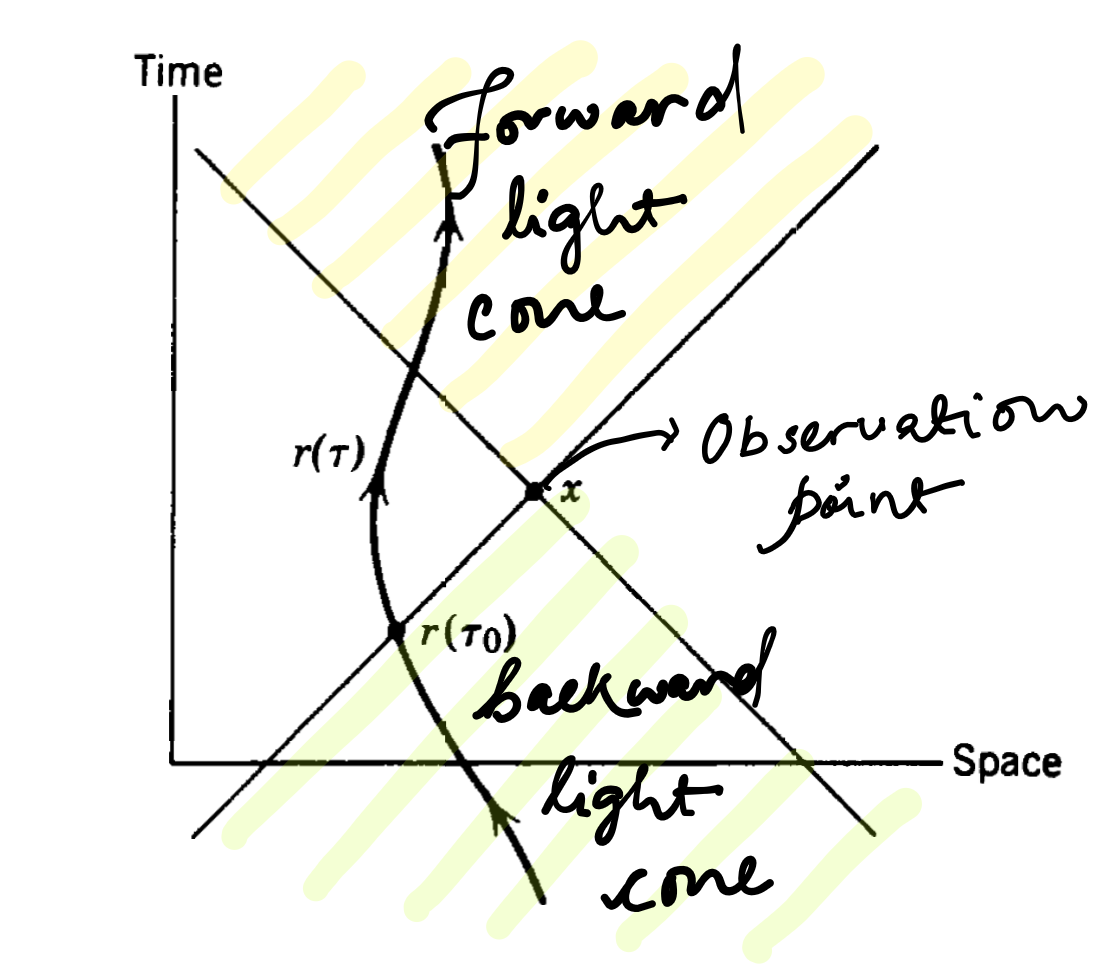
\includegraphics[width=0.7\linewidth]{lienardpot.png}
\label{radlineard}
\end{figure}
Now, focus on Fig. \ref{radlineard}. 
\begin{itemize}
\item Green Function is different from zero only on the backward lightcone of the observation point.
\item World line of the particle, $r(\tau)$, intersects the light cone at only two observation point, one earlier and one later than $x_0$.
\item Consequently in the earlier part, $r^\alpha(\tau_0)$ is the only part of the path that contributes to the field at $x^\alpha$.
\end{itemize}
Now, we know that
\begin{equation}\label{deltatau}
\delta[f(x)]=\sum_i \frac{\delta(x-x_i)}{|\cc{\pe{f}{x}}_{(x=x_i)}|}
\end{equation}
\textbf{Note:} Here, it was assumed that the zeros of $f(x)$ at $(x=x_i)$ are all linear.\\
and also we also need,
\begin{equation}
\frac{d}{d\tau}\rr{x-r(\tau)}^2 =2\rr{x-r(\tau)}_\beta \cc{-\frac{d r(\tau)}{d\tau}}^\beta=-2\rr{x-r(\tau)}_\beta V^\beta(\tau)
\end{equation}
which is evaluated at point $\tau=\tau_0$
\textbf{So, can we say that the motion of charged particle $r(\tau)$ is completely determined by the potential term?}

In our case, $\rr{x-r(\tau)}^2$ is function of $\tau$. In our case, only earlier point contributes to the path, so we consider only $r^\alpha(\tau_0)$ as zeros for \eqref{deltatau}.\\
Therefore, we have,
\begin{equation}\label{deltatau}
\delta([x-r(\tau)]^2)= \frac{\delta(x-r(\tau))}{|-2\rr{x-r(\tau)}_\beta V^\beta(\tau)|_{\tau=(\tau_0)}}
\end{equation}
Now, putting everything in \eqref{Vpotf}:
\begin{eqnarray*}
A^\alpha(x)=2e\int d\tau V^\alpha(\tau)\theta\rr{x_0-r_0(\tau)}\delta\rr{x-r(\tau)}^2\\
=2e\int d\tau V^\alpha(\tau)\theta\rr{x_0-r_0(\tau)}\frac{\delta(x-r(\tau))}{|-2\rr{x-r(\tau)}_\beta V^\beta(\tau)|_{\tau=(\tau_0)}}
\end{eqnarray*}
\begin{equation}
\implies A^\alpha(x)=\frac{e V^\alpha(\tau)}{\rr{x-r(\tau)}_\beta V^\beta(\tau)}|_{\tau=(\tau_0)}\\
\end{equation}
or,
\begin{equation}\label{liendardVpot}
\implies A^\alpha(x)=\frac{e V^\alpha(\tau)}{V . \rr{x-r(\tau)}}|_{\tau=(\tau_0)}
\end{equation}
where, \textbf{$\tau_0$ is defined by \eqref{lc} and Retardation requirement}. And \textbf{\eqref{liendardVpot} is called \tit{Lienard-Wiechert potentials}}.
We can further work on it. Now, Let:
\begin{equation}
x_0-r_0(\tau_0) = \mbf{|x_0-r_0(\tau_0)|} \equiv R
\end{equation}
Hence,
we can write:
\begin{eqnarray*}
\text{First we expand the individual 4 vector components of V.(x-r)}\\
V.(x-r)=V_0\rr{x_0-r_0(\tau_0)}-\mbf{V.\rr{x-r(\tau_0)}}
=\gamma cR-\gamma\mbf{v.n}R\\
\text{where, $\mbf{n}$ is a unit vector in the direction of}\\
\text{$\mbf{x-r(\tau)}$ and $\mbf{\beta=v(\tau)/c}$}\\
\implies \gamma c R(1-\mbf{\beta .n})
\end{eqnarray*}
Finally, we can wite the potential in the final form can be deomposed into components as
\begin{equation*}
 A^\alpha(x)=\frac{e V^\alpha(\tau)}{V . \rr{x-r(\tau)}}|_{\tau=(\tau_0)}
\end{equation*}

\section{Synchrotron Radiation: Basics}
Synchrotron radiation is emitted by charges spiralling in a magnetic field moving at relativistic speeds.\\
\textbf{Why is it important?}\\
Synchrotron has a broad frequency spectrum often corresponding to a million harmonics of the basic frequency of particle in motion.\\


A charged particle in constant magnetic field moves in a circular trajectory in plane perpendicular to $\mbf{B}$.\\
The angular velocity of such a particle with an energy E. If $v.\mbf{B}=0$, then particle moves in a circular path of radius
\begin{equation}
r_B=\frac{v}{\omega}=\frac{mcv}{qB}\gamma
\end{equation}
Before, we start with the business of Synchrotron. We first recapitulate the Synchrotron for non-relativistic electrons. \\

\begin{\cbox}
For non relativistic electrons accelerated by magnetic fields are said to emit cyclotron radiation. The radiation is at frequency of gyration $\omega=eB/m_ec$. 
\end{\cbox}
\textbf{For relativistic particles, this emission extends to higher frequencies and we call it Synchrotron Emission.}

\chapter{Continuum Radiation Processes}
\textbf{This Chapter is largely based on Klein Fetcher's book on galactic and intergalactic magnetic field, Chapter 2. The important point to note is, we will be doing the mathematical part behind radiation in our own time. This is a more applicative based study and less mathematical.}\\
\section{Introduction}
\textbf{Why is studying Sychrotron Radiation important?:}\\
We observe low frequency synchrotron radiation on galactic scales when relativistic electrons move in a magnetic field.\\ 
Studying synchrotron helps us to use it as a tool to trace magnetic fields in interstellar and intergalactic scales, by virtue of its \textbf{radiation spectrum and polarisation properties}.\\

\textbf{What is the issue with observing this low frequency radiation?}\\
The main point of concern is at radio frequency we not only observe the synchrotron radiation, it is contaminated by free-free radiation coming from \textbf{ionised HII regions} and \textbf{ionised medium of milky way} galaxy and other galaxy.\\

So it becomes important for us to know both \textbf{thermal(free-free)} and \textbf{non thermal(synchrotron)} part of energy so that we can extract out the non thermal component.\\
\begin{\cbox}
Free-Free is called thermal radiation because it results from an ensemble of particles with a \textbf{Maxwellian Energy Distribution}. On the other hand, energy distribution of synchrotron follows a power-law.
\end{\cbox}
\begin{\cbox}
Note point: In order to produce measurable Synchrotron radiation vs measurable thermal radiation, the number of relativistic particles required is less lower than the thermal ones. \textbf{Just because they are so energetic} 
\end{\cbox}
\section{Radiation of an Accelerated Electron}
\begin{figure}[th]
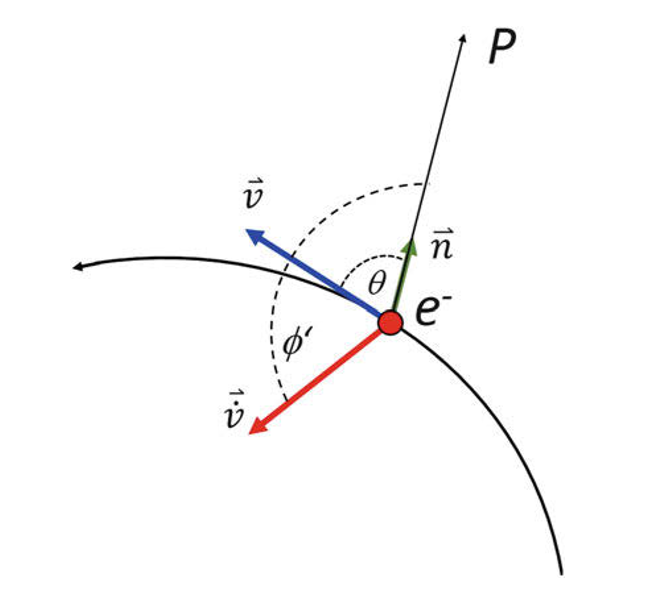
\includegraphics[scale=0.7]{singleprad.png}\label{singleprad}
\caption{Geometry for a moving charged particle as seen from the point P}
\end{figure}
\textbf{What is the electric field for an accelerated electron?}\\
So we have an accelerated electron as Fig. \ref{singleprad}. The velocity of the electron is $\vec{v}$ and the acceleration is $\vec{\dot{v}}$, as seen by observer at some point P. \textbf{Refer Chapter 14 Jackson} The electric field for such a particle is given as
\begin{equation}
\vec{E}=\cc{\frac{e}{c}}\cdot \frac{\vec{n}\times \rr{\cc{\vec{n}-\vec{\beta}}\times \vec{\dot{\beta}}\;}}{R\cc{1-\cos\theta \cdot \beta}^3}
\end{equation}
\begin{itemize}
\item $\vec{n}$ is unit vector pointing from the particle towards the observer.
\item $\beta=\frac{\vec{v}}{c}$ and $\vd{\beta}=\frac{\vd{v}}{c}$
\end{itemize}

\textbf{What is the flux of radiation and the power radiated?}\\
The flux of radiation is given by \textbf{Pontying Vector}
\begin{equation}
\vec{S}=\frac{c}{4\pi}\cdot \vec{E}\times\vec{B}=\frac{c}{4\pi}\cdot |\vec{E^2}|.\vec{n}
\end{equation}
The \textbf{power radiated into a unit solid angle per unit frequency and unit time} Units=[$Wstr^{-1}Hz^{-1}sec^{-1}$] is given by:
\begin{align}
\frac{dP(t)}{d\Omega}&=&|\vec{S}|\cdot(1-\beta \cos \theta)R^2\\
&=&\frac{e^2}{4 \pi c}\cdot \frac{|\vec{n}\times\rr{\vec{n}-\vec{\beta}}\times\vd{\beta}|^2}{(1-\beta \cdot \cos \theta)^5}
\end{align}
R being the distance between observer at point P and the electron.\\
The above equation will be used in the following case and form:
\begin{itemize}
\item $\beta<<1$ for  thermal radiation
\item $\beta\leq 1$ for non-thermal radiation
\end{itemize}
In order to find the power the above equation has to be modified over the $4\pi$ solid angle of the sphere. \textbf{Here, $\theta=\angle (\vec{v},\vec{n})$} and hence
\begin{equation*}
\cos \theta = \vec{n} \cdot \vec{\beta}
\end{equation*}
\begin{\cbox}
When measuring flux densities of radio sources, we can calculate their radio power or luminosity once we can determine this distance using standard astronomical techniques.Hence R is not relevant in the derivations that we shall work out below. It is just a matter of conversion from flux density to power or monochromatic luminosity, or from flux to total power or luminosity. So, converting for instance flux density $S_\nu$ to power $P_\nu$ then reads
\begin{equation*}
P_\nu=4 \pi R^2 S_\nu
\end{equation*}
Assuming the radio source emits isotropically.
\end{\cbox}
\textbf{Skipping the section on free-free Radiation for now!}
\section{Synchrotron Radiation}
\textbf{Why is Synchrotron radiation important? }\\
It basically serves as a diagnostic tool to trace magnetic fields in the ISM and IGM. \\
\textbf{How are the electrons in IGM and ISM are relativistically energised?}\\
\begin{itemize}
\item Electrons are energised in ISM by the shock waves produced during supernovae explosions\\
\item and energised due to AGN activity, by galactic wakes\fn{it is the hypersonic flow of intergalactic gas past a galaxy. \textbf{not sure!!} } and by merging of galaxies for the case of IGM.
\end{itemize}
\textbf{A brief overview:}
\begin{itemize}
\item Relativistic electrons in magnetic field experience Lorentz force.
\item This force makes the particles move in helical motion.
\item This accelerated helical motion leads to synchrotron radiation.
\item This radiation has a characteristics frequency spectrum and is \textbf{partially polarised.}
\end{itemize}
\begin{\cbox}
 galaxies and AGN exhibit synchrotron radiation as soon as they come into existence, a mere few hundred million years after the Big Bang. In fact, the distribution of faint(hence distant)radio sources is characterised by near isotropy,in accord with the cosmological principle. The bulk of these sources are AGN, which may produce Doppler boosting, which renders them detectable out to cosmological distances. 
\end{\cbox}
Another important observable is Faraday Rotation is \textbf{Faraday Rotation} - It allows us to estimate \textbf{Magnetic field strength} and \textbf{and their orientation} (towards and away from us) in the medium towards the radio source.
\subsection{Radiation from a single electron}
So as we already know power radiated from a single relativistic particle into a unit solid angle per unit frequency and per unit time is given by \eqref{eq:rel1particle}
\begin{figure}[h!]
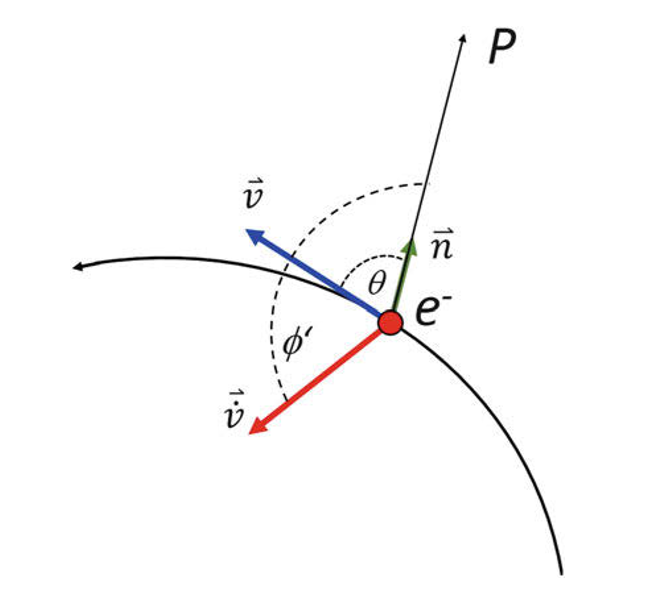
\includegraphics[height=4cm,width=9cm]{singleprad.png}
\caption{Geometry for a moving charged particle as seen from the point P}
\end{figure}

\begin{equation}\label{eq:rel1particle}
\de{P}{\Omega}=\frac{e^2}{4 \pi c} \cdot \frac{|\vec{n}\times \rr{(\vec{n}-\vec{\beta})\times\dot{\vec{\beta}}}|^2}{(1- \vec{n}\cdot \vec{\beta})^5}
\end{equation}
\begin{itemize}
\item $\vec{n}$ is unit vector pointing from the particle towards the observer.
\item $\beta=\frac{\vec{v}}{c}$ and $\vd{\beta}=\frac{\vd{v}}{c}$
\end{itemize}
When dealing with relativistic particles, we study two cases of the direction of $\vd{\beta}$ and $\beta$.
\begin{enumerate}
\item \tbf{LINEAR ACCELERATOR or }($\vd{\beta} \parallel \beta$):
Then we have the power radiated derived from \eqref{eq:rel1particle} to be :
\begin{equation}\label{eq:rel1particlelin}
\de{P}{\Omega}=\frac{e^2 \dot{v^2}}{4 \pi c} \cdot \frac{\sin^2 \theta}{(1- \cos \theta \beta)^5}
\end{equation}
\tbf{It is to be noted that:the radiation pattern has a strong dependence on the angle  and on the particle speed}. Refer to book to check out how $\beta$ influences radiation pattern. \tbf{\tit{What do we mean when we say radiation pattern, what are we plotting?}}.
The reason for strong dependence of value of $\beta$ on radiation pattern is because the maximum power radiated depends on $\gamma$ i.e.
\begin{equation}
\de{P}{\Omega}(\theta_{max}) \sim \gamma^8
\end{equation}
where,
\begin{equation}
\cos \theta_{max}=\frac{1}{3 \beta}\cc{\sqrt{1+15 \beta^2}-1}
\end{equation}
The above equations can be obtained by maximizing equation \eqref{eq:rel1particlelin} with respect to $\theta$ and then substituting  back in \eqref{eq:rel1particlelin} and $\theta_{max}=\frac{1}{2\gamma}$ i.e. is the maximum power is radiated when $\theta$ is very small and photons are emitted in the direction of acceleration.
\begin{\cbox}
The strong dependence on the Lorentz factor is called 'relativistic boosting' or 'beaming', meaning that a charged particle moving with relativistic speed emits essentially its whole radiation in the forward direction. 
\end{\cbox} 

The total radiation of the relativistic particle is given by the integration:
\begin{eqnarray*}
P(t)=\int^{2\pi} _{0} \int^{\pi} _{0} \de{P}{\Omega} d\Omega \\
\implies P(t)=\int^{2\pi} _{0} \int^{\pi} _{0} \frac{e^2 \dot{v^2}}{4 \pi c} \cdot \frac{\sin^2 \theta}{(1- \cos \theta \beta)^5} \sin^2 \theta d\theta d\phi \\
\implies P(t)= \frac{e^2 \dot{v^2}}{2 c} \int^{\pi} _{0}  \frac{\sin^2 \theta}{(1- \cos \theta \beta)^5} \sin^2 \theta d\theta \\
\implies P(t)=\frac{2}{3}\cdot \frac{e^2 \dot{v^2}}{c^3} \cdot \gamma^6
\end{eqnarray*}

\item \tbf{Transverse or CYCLOTRON ACCELERATOR or SYNCHROTRON }($\vd{\beta} \perp \beta$): Check Figure \ref{figtrac}. The geometry of and various angle required are given in right hand cartoon and the left hand cartoon refers to the same particle moving in interstellar magnetic field. 
\begin{figure}[h!]\label{figtrac}
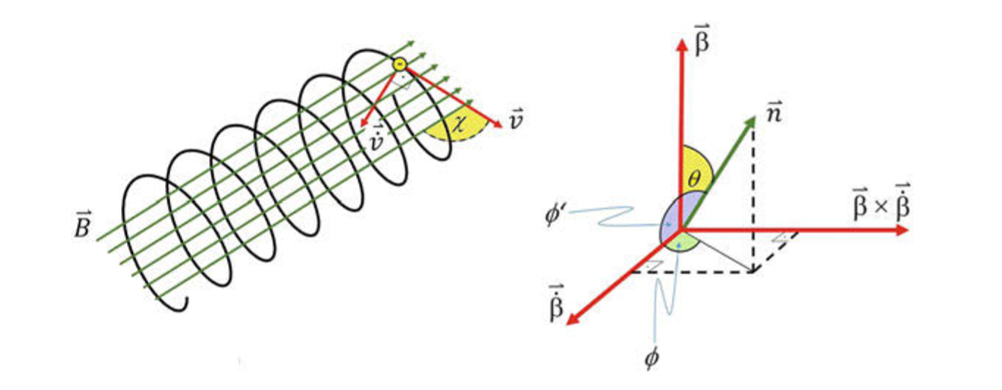
\includegraphics[scale=1]{figtrac}
\caption{ Illustration of the various angles used in describing the transverse acceleration of a relativistic electron in a magnetic field}
\end{figure}
\end{enumerate}
\textbf{Define Pitch angle:}\\
Pitch angle is the motion of particle is inclined to the magnetic field vector. In Figure \ref{figtrac} $\chi$ is the \textbf{pitch angle}.\\

 Now the, particle experiences \textbf{Lorentz force} and $\vec{\beta} \perp \vd{\beta}$ and 
\begin{eqnarray}
\de{P}{\Omega}=\frac{e^2}{4 \pi c} \cdot \frac{|\vec{n}\times \rr{(\vec{n}-\vec{\beta})\times\dot{\vec{\beta}}}|^2}{(1- \vec{n}\cdot \vec{\beta})^5}
\implies \de{P}{\Omega}=\frac{e^2 \dot{v^2}}{4 \pi c^3} \cdot \frac{1-\frac{\sin^2 \theta \cos^2 \phi }{\gamma^2(1-\beta \cos \theta)^2}}{(1-\beta \cos \theta)^3}
\end{eqnarray}
\textbf{As in case of the linear accelerator, the relativistic motion causes a relativistic aberration of the radiation of the charged particle, i.e. a strong distortion of the radiation pattern. check Figure \ref{figtracpa}}
\begin{figure}[h!]\label{figtracpa}
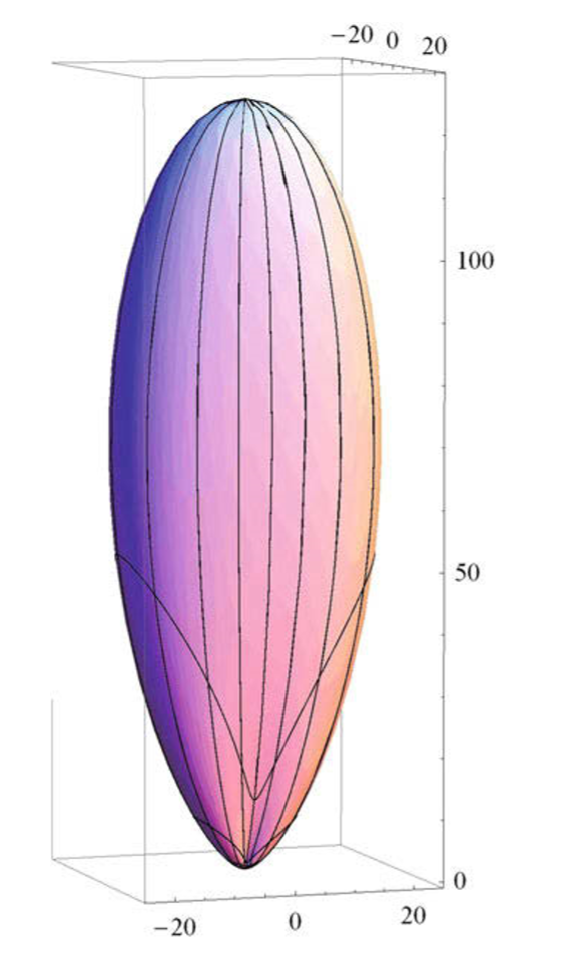
\includegraphics[scale=1]{figtracpa.png}
\caption{Radiation pattern of the transversely accelerated electron ($\beta$:0.8)}
\end{figure}
\textbf{Its main lobe can be shown to have a half-power width that is inversely proportional to the Lorentz factor 1=$1/\gamma$ at half-maximum} or 
\begin{equation}
\theta_{HP}\approx 1/\gamma =\frac{m_0c^2}{E^2}
\end{equation}
Note:The half-power width is the angular width of the radiation  pattern at which the power has dropped to half its maximum value.\\
\textbf{As in case of the transverse accelerator, the radiated power has a strong dependence on the Lorentz factor:
\begin{equation}
\de{P}{\Omega} \sim \dot{v^2}\gamma^6
\end{equation}
and
\begin{equation}
P(t)=\int^{2 \pi} _{0}\int^{ \pi} _{0} \de{P}{\Omega} d\Omega \sim \dot{v^2}\gamma^4
\end{equation}
}

Now, we try to calculate the Larmor Circle and at the end of it you would understand why we need it at all:\\
Now, the equation of motion a charged particle in magnetic field is given by
\begin{equation}
m\vd{v}=m\cdot (\vec{v}\times \vec{\omega_L})=\frac{-e}{c}(\vec{v}\times \vec{B})
\end{equation}
Let us consider the pitch angle, $\chi=90^circ$ i.e. the particle motion is perpendicular to the magnetic field.Hence,
\begin{eqnarray}
m\omega^2_Lr_L=m\cdot \frac{v^2}{r_L}=\frac{e}{c} \cdot vB
\implies m\frac{v}{r_L}=\frac{e}{c} B\\
\implies \omega_L=\frac{eB}{mc}
\end{eqnarray}
Now for a relativistic particle we know, $m=\gamma m_0$, since $E=mc^2=\gamma m_0c^2$. Therefore,
\begin{equation}
\omega_L=\frac{eB}{mc}
\end{equation}
and the larmor radius for $v\approx c$ is
\begin{equation}
r_L=\frac{v}{\omega_L}=\frac{m_0vc}{eB}\cdot \gamma\approx \frac{m_0c^2}{eB}\cdot \gamma =\frac{E}{eB}
\end{equation}
or in general,
\begin{\cbox}
\begin{equation}
r_L=\frac{E}{eB}\sin \chi
\end{equation}
We realise that the Larmor radius does not depend on the mass of the particle, but just on its energy (and on the magnetic- field strength). 
\end{\cbox}
Now, for a $\gamma=1$ and a magnetic field of $B=10\mu G$ we have a frequency of 28Hz. 
\textbf{Now, the question may be asked that how can we observe such particles in radio regime? The answer to this question is in}

\begin{\cbox}
\textbf{what we have found is the power emitted by the relativistic particle in the direction of observer, but we need to make a frame transition to observer's frame if we want to obtain power spectrum seen by the observer}
\end{\cbox}
Therefore, the way the observer observes the radiation from electron is is by calculating the time dependence of radiation as seen by the observer.\\
Now, in order to calculate the radiation spectrum \textbf{ we perform a Fourier analysis of the time-dependent radiation power of single particles,then 'fold in' their energy spectrum and then calculate the emissivity.} The frequency of the emitted pulses of the gyrating relativistic electrons \textbf{ corresponds to the inverse of the time that the radiation pattern needs to sweep across the observer}.
Therefore, we can visualize the radiation emitted by the particle as given in Fig. \ref{figobsrad}
\begin{figure}\label{figobsrad}
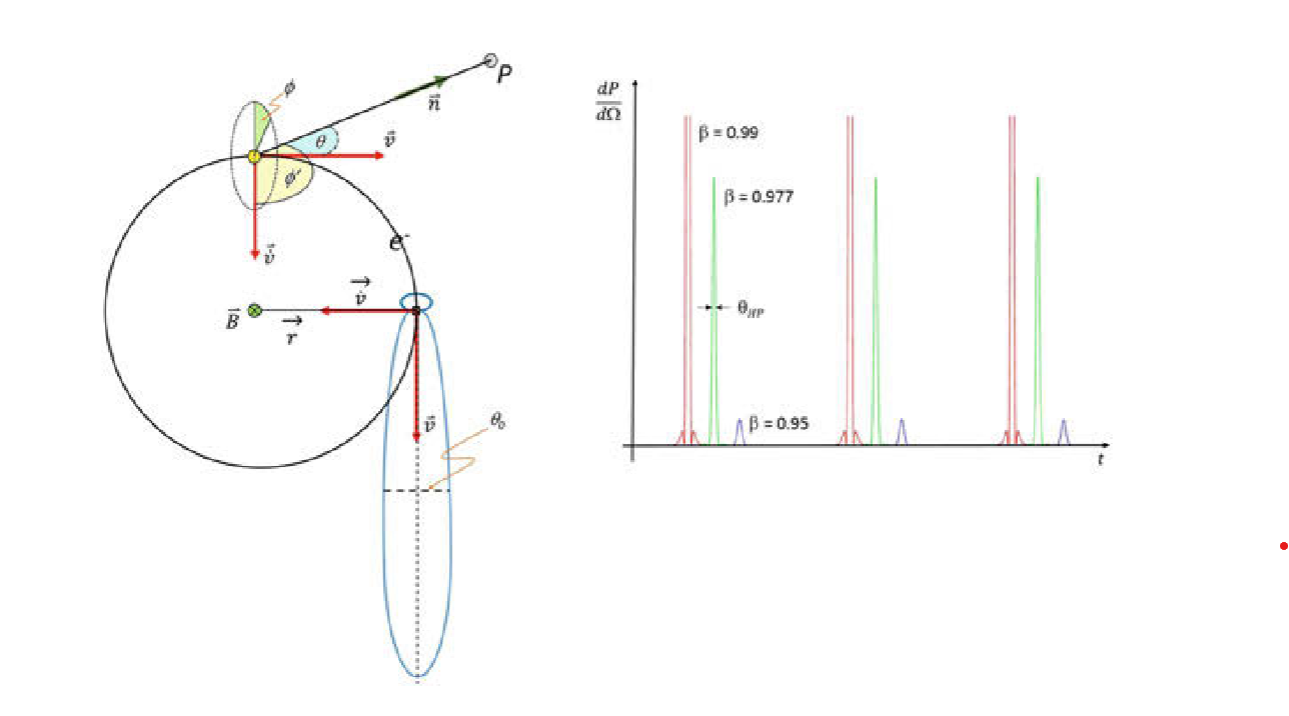
\includegraphics[scale=1]{figobsrad.png}
\end{figure}
\textbf{Now, how long does the pulse last in particle's frame of reference:}\\
The duration of the pulse in the particle's frame of reference is equal to:
\begin{equation}
\Delta t =\frac{r_L\theta_{HP}}{v}\approx \frac{r_L \theta_{HP}}{c}
\end{equation}
and since, $r_L \approx \frac{Ee}{B}$ and $\theta_{HP}\approx \frac{1}{\gamma}$, we find 
\begin{equation}
\Delta t =\frac{m_0 c}{e B}
\end{equation}
Our next order of business would be transforming frames from particles to observer i.e. from t frame to $t^\prime$.\\
The transformation is shown in Figure \ref{figtrans}. What we need to account is the motion of particle when it emitted the pulse of duration $\Delta t$. Therefore our transformation time is given as 

\begin{figure}[h!]\label{figtrans}
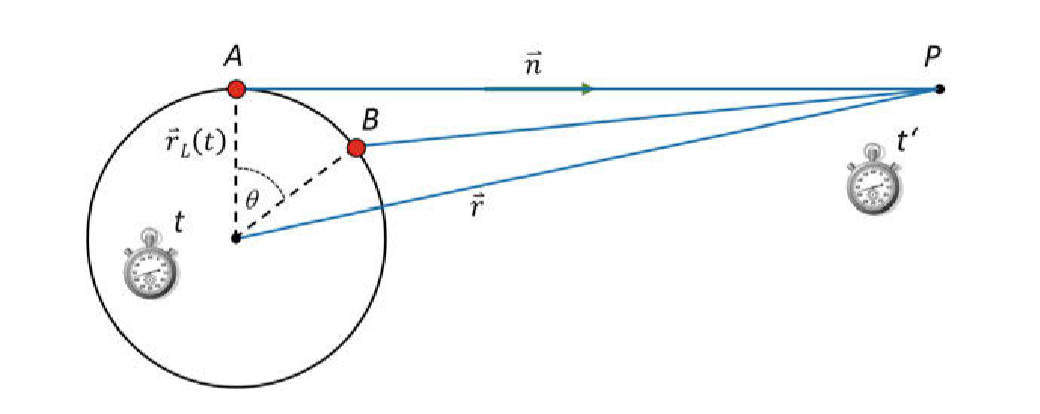
\includegraphics[width=\linewidth]{figtrans.png}
\caption{geometry of the transformation from the particle's to the observer's reference frame}
\end{figure}
\begin{equation}
t^\prime=t+\frac{|\vec{r}-\vec{r_L(t)}|}{c}
\end{equation}
Now, the rate of change of time in one frame to another is given as follows:
\begin{eqnarray*}
t^\prime=t+\frac{|\vec{r}-\vec{r_L(t)}|}{c}\\
\implies t^\prime=t+\frac{\cc{\cc{|\vec{r}-\vec{r_L(t)}|}^2}^{1/2}}{c}\\
\implies \de{t^\prime}{t}=1-\frac{\vec{r}-\vec{r_L(t)}}{|\vec{r}-\vec{r_L(t)}|}\cdot \de{\vec{r_L(t)}}{t}\\
\implies \de{t^\prime}{t}=1-\frac{\vec{n}\cdot \vec{v}}{c}=1-\beta \cdot \cos \theta_{HP}\\
\tx{I think $\theta_{HP}$ is the average value of angle between $\vec{n}$ and $\vec{v}$}\\
\tx{and, for small angles}\\
\implies \de{t^\prime}{t}=1-\beta \cdot \sqrt{1- \theta^2_{HP}} \\
\implies \de{t^\prime}{t}=1-\beta \cdot \sqrt{1- \frac{1}{\gamma^2}} \\
\implies \de{t^\prime}{t}=1-\beta^2 =\frac{1}{\gamma^2} \\
\end{eqnarray*}
\begin{\cbox}
\begin{equation}
\Delta t^\prime =\frac{\Delta t }{\gamma^2}
\end{equation}

\end{\cbox}
Now, Remember the argument of particle emitting at frequency 28Hz at $B=10\mu G$, for $\gamma=2000$, the frequency spectrum is shifted towards a $\gamma^2$ higher range and that would be around $\nu=700MHz$.\\
Now we define \tbf{a critical frequency} and the purpose of this being \tbf{the particles produce a significant power at this frequency}. given as $\omega_c =2 \pi \nu_c$. Even though $\omega_c$ has different definitions, we will use one by Schwinger 
\begin{equation}
\omega_c\equiv \frac{1}{\frac{2}{3}\Delta t^\prime}
\end{equation}
and substituting the value of $\Delta t$ here we get
\begin{\cbox}
\begin{equation}
\nu_c=\frac{3}{4 \pi}\cdot \frac{e B_{\perp}}{m_0c}\cdot \gamma^2
\end{equation}
Here, $B_{\perp}=B \cdot \sin \chi$. is the component of the magnetic field perpendicular to the line-of-sight.
\end{\cbox}
\textbf{So far so good, we have considered the synchrotron emission from particles composed of only electrons. What about protons? Evidently, The cosmic-ray (CR) energy spectrum observed near earth exhibits $\sim 100$ times more protons than electrons (at the same energy).}\\
Here, we now check for the contribution of protons:\\
So, we know,
\begin{equation}
\nu_c=\frac{3}{4 \pi}\cdot \frac{e B_{\perp}}{m_0c}\cdot \gamma^2
\end{equation}
We substitute $\gamma= \frac{E}{m_0c^2}$. 
\textbf{This tells us a crucial fact, $\nu_c$ depends on the mass of the radiating particle like $m^{-3}$}. And, we can find that
\begin{equation}
\cc{\frac{m_p}{m_e}}^{-3}=1.6 \cdot 10^{-10}
\end{equation}
and hence the frequency for proton relative to electron would be around
\begin{equation}
\cc{\frac{\nu_{c,p}}{\nu_{c,e^{-1}}}}=1.6 \cdot 10^{-10}
\end{equation}
\textbf{Put differently, we can calculate how much more kinetic energy a proton must have in order to radiate at the same frequency as the electron.}
\begin{equation}
E_p=\cc{\frac{m_p}{m_e}}^{3/2}\cdot E_e =8\cdot 10^4 E_e
\end{equation}
\textbf{Hence, even the ratio of number densities measured in the CR energy spectrum of $np/ne \approx 100$ does not help. In fact, as we shall see later, \tit{relativistic protons are much more long-lived, owing to their very low radiation losses. They may remain relativistic for more than a Hubble time, while electrons become non-relativistic within less than 100 Myr}}\\
Remember the power of the time dependent radiated power into a unit solid angle per unit frequency and per unit time is
\begin{align}
\frac{dP(t)}{d\Omega}&=&\frac{e^2}{4 \pi c}\cdot \frac{|\vec{n}\times\rr{\vec{n}-\vec{\beta}}\times\vd{\beta}|^2}{(1-\beta \cdot \cos \theta)^5}
\end{align}
For, small angle $\theta$ and large Lorentz factors $\gamma$\textbf{Note: I have not done this calculation yet.}
\begin{equation}
frac{dP(t)}{d\Omega}=\frac{2}{\pi}\;\frac{e^2 \dot{v}^2}{c^3} \gamma^6\cdot \frac{1}{(1+\gamma^2 \theta^2)^3}\cdot \rr{1-\frac{4 \gamma^2 \theta^2 \cos^2 \phi}{(1+\gamma^2\theta^2)^2}}
\end{equation}
and, upon integration over solid angle it becomes
\begin{equation}\label{eq:timeP}
P(t)=\int^{2 \pi}_0 \int^{\pi}_0 \de{P}{\Omega}d\Omega=\frac{2}{3}\frac{e^2\dot{v}^2}{c^3}\cdot\gamma^4
\end{equation}
Now, what we do is the \tbf{Fourier analysis of time-dependent radiated power} for the small angle approximation [\textbf{Done by schwinger}]:
\begin{equation}
P(\nu)=\frac{\sqrt{3}e^3}{m_0 c^2} \cdot B_{\perp} \cdot F\cc{\frac{\nu}{\nu_c}}
\end{equation}
where
\begin{equation}\label{eq:freqP}
F\cc{\frac{\nu}{\nu_c}}=\frac{\nu}{\nu_c}\cdot \int^\infty_{\nu/\nu_c} K_{5/3}(x)dx
\end{equation}
\textbf{The function $F\cc{\frac{\nu}{\nu_c}}$ is the Airy integral of the modified Bessel Function $K_{5/3}(x)$}. Th Wallis approximation renders us the following important result
\begin{\cbox}

\begin{equation}
F\cc{\frac{\nu}{\nu_c}}=1.78 \cc{\frac{\nu}{\nu_c}}^{0.3} \cdot e^{-\frac{\nu}{\nu_c}} 
\end{equation}
\end{\cbox}
Using \eqref{eq:timeP} and \eqref{eq:freqP} we can plot for various values of $\gamma$ as given in Figure \ref{figfour}

\begin{figure}\label{figfour}
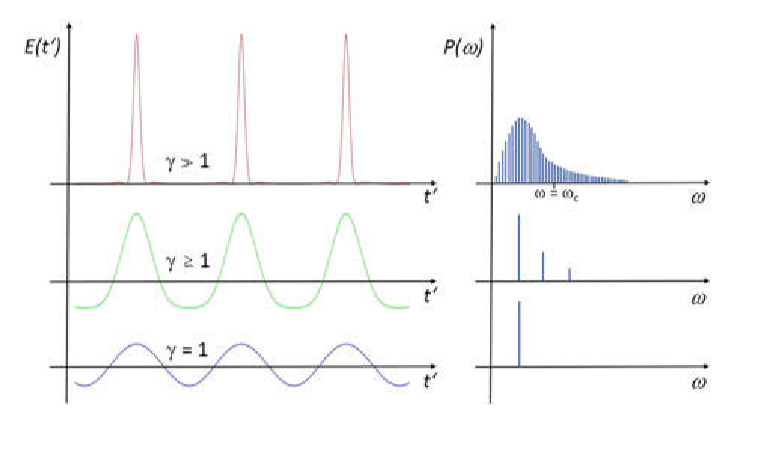
\includegraphics[scale=1]{figfour.png}
\caption{Sketch of the time dependence of the synchrotron pulses and their radiation spectra}
\end{figure}

\subsection{Synchrotron Radiation from Relativistic Electrons with an Energy Spectrum}
Now, if we need to measure the radiation coming in from a bunch of particles we would need to know the energy spectrum of the bunch of charges. The CR shower on the atmosphere has been observed and identified to follow as power lay given as given as
\begin{equation}
N(E)dE=A\cdot E^{-g}dE
\end{equation}
and plotted in Figure \ref{figepower} which shows the measured energy spectrum near earth.
\begin{figure}\label{figepower}
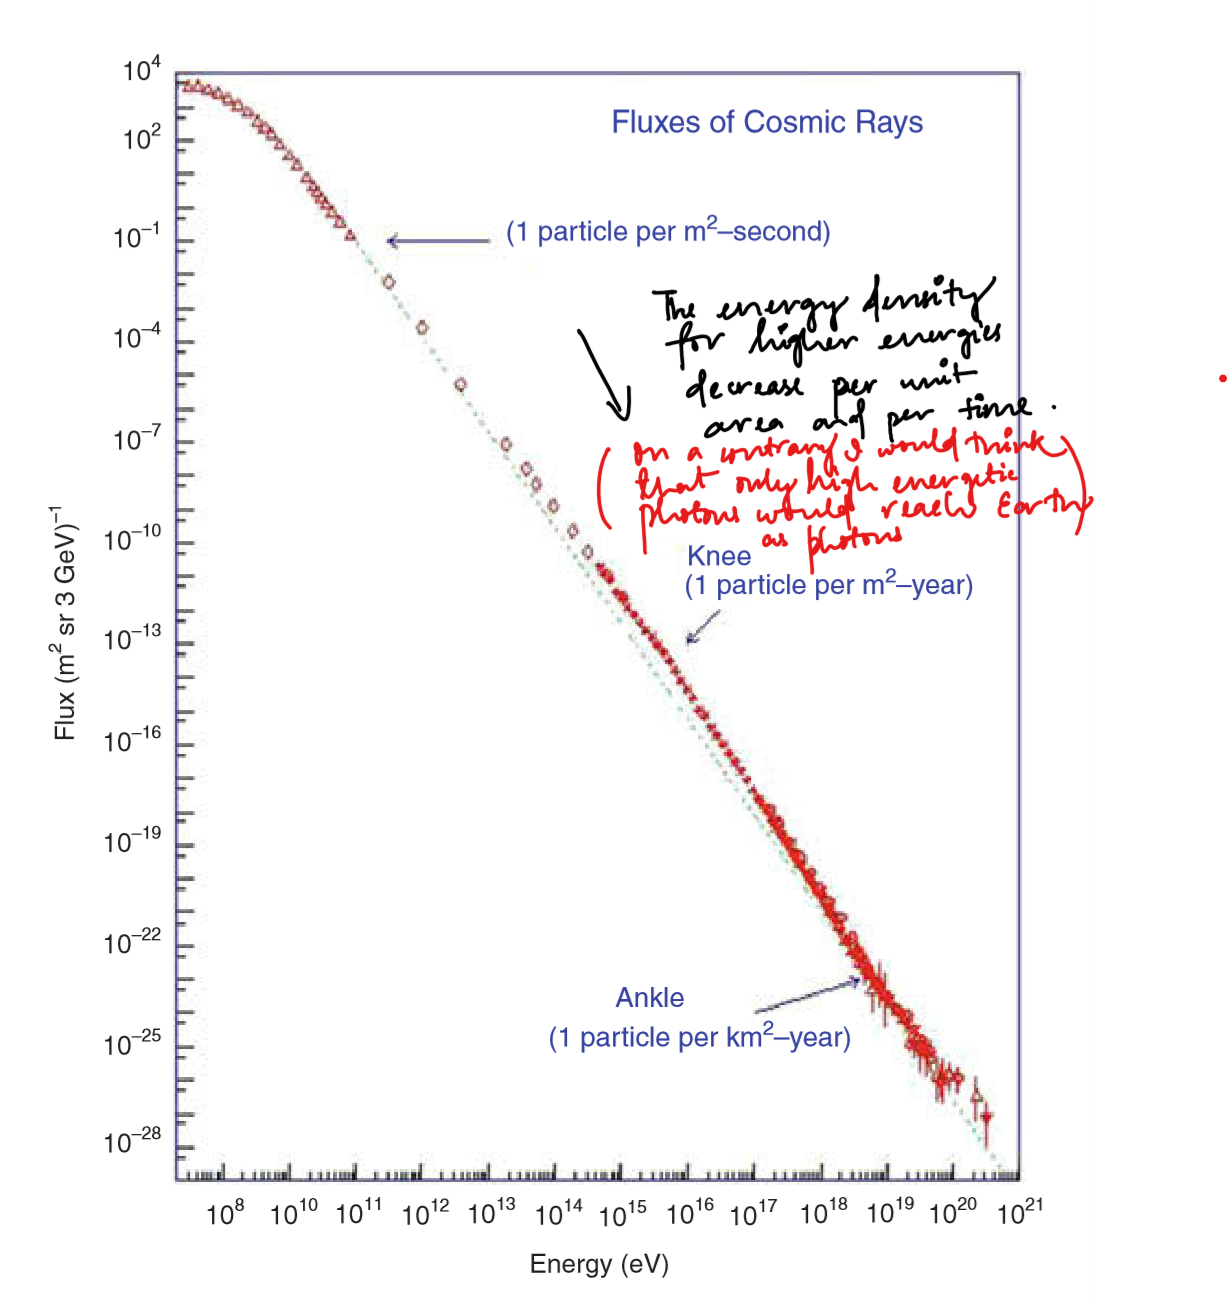
\includegraphics[scale=1]{figepower.png}
\end{figure}
\begin{itemize}
\item A is a constant. Representing the local number density of relativistic particles per energy interval.
\item g is the power law index , \textbf{generally g=2.4}
\end{itemize}
Coming back to Figure \ref{figepower}:
\begin{itemize}
\item ($\leq 1GeV - 10's\;\;GeV$): Represents energies of particles emitting synchrotron
\item  measured spectrum is strongly modulated by the solar wind below a few GeV, which explains the deviation from the power-law there. Hence, nothing is known about the shape of the spectrum at the lowest CR energies. 
\item  At the highest energies, there are changes in the spectrum called 'knee' (at $\geq 10^{15}$ eV) and 'ankle' (at $\geq 10^{18}$ eV).
\item  The particles with the highest recorded energies($\geq 10^{20}$ eV, so-called ultra-high energy cosmic rays, or UHECR) are a real enigma, their origin being totally unknown.

\end{itemize}
Now, the intensity of emission is given through the emissivity equation:
\begin{equation}
4 \pi \epsilon_\nu=\int^{E_2}_{E_1}P(\nu)\cdot N(E)dE
\end{equation}
\textbf{Assuming that there is no background radiation, the radiation transport equation yields the intensity from the brightness and the source function}
\begin{equation}
I_\nu=S_\nu(T)\cdot (1-\exp^{-\tau_\nu}) \approx S_\nu(T)\cdot \tau_\nu
\end{equation}
for small values of $\tau_\nu$. we expect the medium to more or less transparent to the observed frequency but \textbf{should the $\tau_\nu$ not be tending more toward infinity. then why do we assume that the $\tau_\nu$ is small?}.\\
From Kirchoff's law we have \textbf{Look into this too}
\begin{equation}
S_\nu(T)=\frac{\epsilon_\nu}{\chi_\nu}
\end{equation}
result in
\begin{equation}
I_\nu=\int^{s_0}_0\epsilon_\nu ds
\end{equation}
and hence
\begin{equation}
I_\nu=\frac{1}{4\pi}\int^{s_0}_0 \int^{\infty}_0 P(\nu) N(E)dEds
\end{equation}
\textbf{check about above definition I am not so sure!!!!}\\
The units of brightness or intensity is given as $\rr{erg\;\;s^{-1}\;\;cm^{-2}\;\;Hz^{-1}\;\;sr^{-1}}$.\\
\tbf{\tit{ Let us assume for simplicity that neither the power $P(\nu)$ nor does the energy spectrum depends on the location.}}\\
i.e. $dP/ds=0$ and $dN/ds=0$.\\
Using the equations of Power in frequency domain and energy spectrum we have
\begin{equation}
I_\nu=\frac{s_0}{4\pi}\cdot \frac{\sqrt{3}e^3}{m_0c^2}\cdot B_{\perp} A \cdot \int^{\infty}_0 F\cc{\frac{\nu}{\nu_c}}E^{-g}dE
\end{equation}
\textbf{$s_0$ being the total path length}.\\
When push in Waalis approximation
\begin{equation}
I_\nu=\frac{s_0}{4\pi}\cdot \frac{\sqrt{3}e^3}{m_0c^2}\cdot B_{\perp} A \cdot 1.78 \cdot \int^{\infty}_0 \cc{\frac{\nu}{\nu_c}}^{0.3} \dot e^{-\nu/\nu_c}E^{-g}dE
\end{equation}
Let's do some assignments for abstraction:
\begin{eqnarray*}
C\equiv 1.78  \frac{\sqrt{3}e^3}{4 \pi m_0c^2}=3.32 \times 10^{-23}esu^3 erg^{-1}\\
\nu_c=\frac{3}{4\pi}\cdot\frac{eB_{\perp}}{m_0^3c^5}\cdot E^2\equiv \eta B_{\perp} E^2\\
\eta=6.26 \times 10^{18}s^4g^{-5/2}cm^{-7/2}
\end{eqnarray*}
We also make use of substitution
\begin{equation}
\sqrt{\frac{\nu_c}{\nu}}\equiv x =\cc{\frac{\eta \cdot \beta}{\nu}}^{1/2}\cdot E
\end{equation}
i.e.
\begin{equation}
dE=\cc{\frac{\nu}{\eta B}}^{1/2}dx
\end{equation}
To be derived:\\
The expression for intensity is given as
\begin{equation}
I_\nu=s_0 C A \eta^{\frac{g-1}{2}}B_{\perp}^{\frac{g+1}{2}}\nu^{\frac{-g+1}{2}}\int^\infty_0 x^{-(g+0.6)}e^{-\frac{1}{^2}}dx
\end{equation}
\begin{\cbox}
Not only for Milky way but even for external galaxies h=2.4
\end{\cbox}
Therefore with
\begin{equation}
\frac{1}{x^2}=u \implies \frac{-2}{x^3}dx=du
\end{equation}
we have
\begin{equation}
\int^\infty_0x^{-3}\cdot e^{-\frac{1}{x^2}}dx=\frac{1}{2}\int^\infty_0 e^{-u}du=\frac{1}{2}
\end{equation}
and using $g=2.4$ we finally have
\begin{\cbox}
\begin{equation}
I_\nu=2.4 \cdot 10^{-10}\cc{\frac{s_0}{cm}}\cc{\frac{A}{erg^{1.4}cm^{-3}}}\cc{\frac{B_\perp}{G}}^{1.7}\cc{\frac{\nu}{Hz}}^{-0.7}
\end{equation}
\end{\cbox}
which has the dimensions of $\rr{erg\;\;s^{-1}\;\;cm^{-2}\;\;Hz^{-1}\;\;sr^{-1}}$.\\
let us look into some numbers first some number crunching, \\
The value of A $=8.2 \times 10^{-17}erf^{1.4}cm^{-3}$ close to earth, this is true. But we take it constant over a line of sight of 10Kpc, then the magnetic field would expect synchrotron intensity as
\begin{equation}
I_\nu \approx 10^{18} erg s^{-1} cm^{-2} Hx^{-1} sr^{-1}
\end{equation} 
at an observing frequency of $\nu =1GHz$.\\
In general if
\begin{\cbox}
The energy spectrum is given by:
\begin{equation}
N(E)dE\sim E^{-g}dE
\end{equation}
then we have
\begin{equation}
I_\nu \sim B_{\perp}^{1+\alpha}\cdot \nu^{-\alpha}
\end{equation}
where $\alpha$ is the spectral index . The spectral index related to the power law index  $g$ as 
\begin{equation}
\alpha=\frac{g-1}{2}
\end{equation}
For ISM, g=2.4 and $\alpha=0.7$.
\end{\cbox}
\textbf{ The synchrotron spectrum steepens in regions of lacking energy supply , while in the vicinity of star-forming regions in which stellar winds and supernovae cause turbulence and (re-)accelerate the particles. What is happening in computing I
is that for each electron the radiation spectrum P($\nu$) of the single particle is successively multiplied by the 'particles' number density for each energy. The integration over the whole energy range then yields the frequency spectrum. In the log-log plot this means that we have to add (logarithmically) the 'weighting functions', given by N(E). \tit{If the energy spectrum has a cut-off at some energy $E_{max}$, the spectrum will fall off exponentially beyond the corresponding critical frequency}}.
\begin{equation}
\nu_c=\frac{3}{4 \pi}\cdot \frac{e. B_{\perp}}{m_0c}\cdot \gamma^2_{max}
\end{equation}
Now, we show an illustration for the cut off frequency and single electron spectrum plot in Figure. \ref{figsyn}
\begin{figure}\label{figsyn}
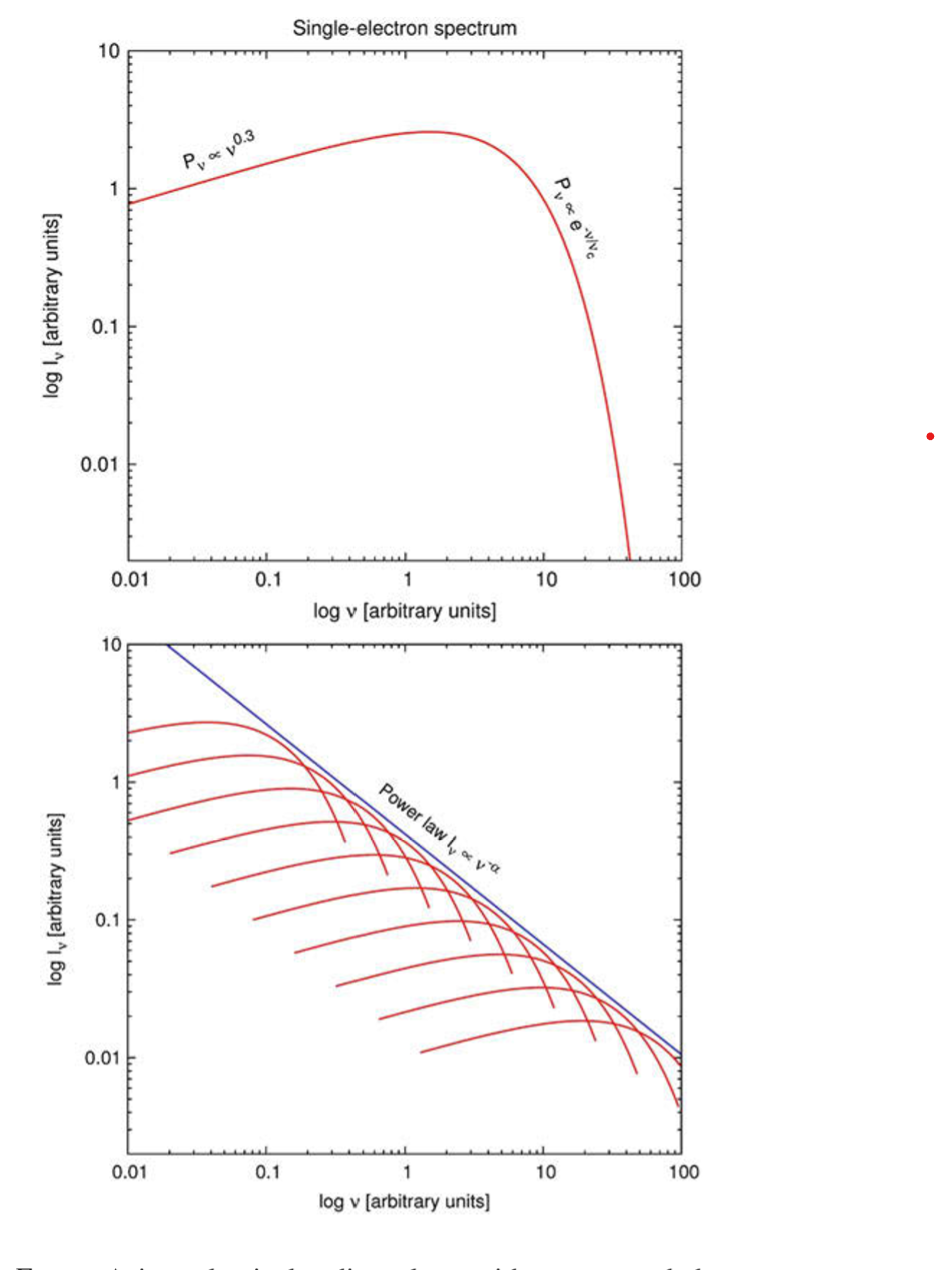
\includegraphics[scale=1]{figsyn.png}
\end{figure}
\chapter{Diffuse Radio Emission from Galaxy Clusters}
\textbf{This work is largely based on R.J.  Van Weeren's review paper with the same title}
\section{Abstract}
With increased detection of galaxy clusters there has been increased identification of the diffuse extended radio sources. \textbf{Note point: These sources may not be individually linked to host cluster galaxies.}And the radio emission from these sources reveal the presence of \textbf{cosmic rays and magnetic fields in the intra-cluster medium (ICM)}\\
\textbf{What comprises of this intra-cluster medium?}\\
\textbf{What are cosmic rays and why are they important at all?}
The diffuse cluster radio sources can be classified as:
\begin{itemize}
\item Radio Halos: They can be further classified as:
\begin{itemize}
\item Giant halos
\item Mini halosa
\item Ans possible intermediate sources
\end{itemize}
\textbf{Where do you find these halos and how does their brightness vary?}\\
 Halos are generally positioned at cluster center and their brightness approximately follows the distribution of the thermal ICM.\\
 \textbf{How are halos formed at cluster center and why is the brightness following the distribution of the thermal ICM?}\\
\item Cluster Radio Shocks(Relics): These are generally found in Cluster's periphery.\\
\textbf{Again, here it becomes important to know how are the relics formed? what do we know about them?}\\
\textbf{\textit{One very crucial property here is they are tracer for merger induced shock waves!!}}
\item Revived AGN fossil plasma sources:\\
\textbf{Among other sources, how do you identify Revived fossil plasma sources?}\\
Ans. \begin{itemize}
\item They have steep radio spectra. I guess in the intensity vs frequency graph, it rises very fast.
\item They have irregular morphologies
\end{itemize}
\end{itemize}
\textbf{What will you study here?}\\
\begin{itemize}
\item We will have an overview of recent results regarding properties of this diffused sources.
\item We will discuss, the resulting implications for the underlying physical acceleration processes that operate in the ICM.
\item we will discuss, the role of relativistic fossil plasma and the properties of ICM shocks and magnetic fields.
\end{itemize}
\newpage
\section{Introduction}
When we talk about scales in universe, galaxy clusters are \textbf{largest virialized objects} objects in the universe. $M_{cluster}=\sim 10^{15} M_\odot$. They grow through the accumulation of smaller groups of galaxies and through major mergers with other massive clusters. Located between clusters, elongated filaments of galaxies, form even larger unbound structures, making up the cosmic web. These filaments span the regions between clusters. 


\textbf{Galaxy clusters are located at the nodes of filaments, like spiders in the cosmic web.}\\
\textbf{What is ICM? What is its emission form like?}\\
Ans. Clusters may contain up to several thousands of galaxies. However, the galaxies comprise \textbf{of only $1\%$ of cluster's total mass}.\\
Most of the baryonic mass is contained in \textbf{hot $(10^7-10^8 \;\; K)$, ionized cluster medium(ICM)} held together by cluster's gravitational pull.\\
\begin{itemize}
\item \textbf{The main emission mechanism is:} Thermal Bremstrahlung at X-ray wavelengths. 
\item \textbf{ The ICM makes up $\sim 15\%$ of a cluster’s mass budget. Most of the mass, $\sim 80\%$, is in the form of dark matter }.
\end{itemize}
Earlier, remember we were talking about the filaments. Now these filaments are surrounded by \textbf{Warm Hot Intergalatic Medium}. Let us compare the properties of ICM and WHIM
\begin{itemize}
\item Particle density: 
\begin{itemize}
\item ICM: $\sim 10^{-3} \text{particle per } cm^{-3}$
\item WHIM: $\sim 10^{-4} \text{particle per } cm^{-3}$
\end{itemize} 
Therefore , WHIM is less dense than ICM.
\item Medium Temperature:
\begin{itemize}
\item ICM: $(10^7 -10^8 \;\ ; K)$
\item WHIM: $(10^5 -10^7 \;\ ; K)$
\end{itemize}
WHIM is hence cooler then ICM.
\end{itemize}
\begin{\cbox}
\textbf{So, fun fact: Half of Universe's baryons reside in WHIM}
\end{\cbox}
\begin{\cbox}
\textbf{Galaxy filaments are expected to be surrounded by accretion shocks, where the plasma is first shock heated!.}\\
\textbf{Why are the filaments expected to be surrounded by shocks?}
\textbf{Q. so if it is said plasma is shock heated, is accretion shock the reason, why ICM has hence higher temperature?}
\end{\cbox}
\textit{studying the WHIM and associated shocks is difficult due to a lack of sensitive observational tools.}\\
\textbf{How are galaxy clusters formed and what are the consequences?}\\
Ans. They are formed by accretion from the WHIM and through a sequence of mergers of clusters and groups. These mergers are highly energetic events, releasing upto $\sim 10^{64} \; ergs\; \text{On a few giga year time scale}$. This energy is dissipated through low Mach number shocks and turbulence,  This strongly affects the physical properties of the different properties of clusters, for example the density distribution and velocity dispersion of galaxies, and the temperature, metallicity, and density distribution of \\
 The shocks and turbulence that are generated in the ICM might also amplify magnetic fields ($\sim \mu G$) and accelerate relativistic particles (Lorentz factor $\gamma >>$  1000), resulting in megaparsec-scale synchrotron emission regions\\
  The spectral index $\alpha$ of the synchrotron emission is generally steep: $\alpha \leq 1$ with $S \propto \nu^\alpha$, where $\nu$ is the observed frequency and S is the measured flux density. The steep spectral index suggests that the synchrotron emission is relatively bright at low radio frequencies. \\
 
\textbf{Q. Is the above mentioned mechanism the only one to heat the ISM, is heating due accretion shock another reason to heat up ICM?}\\
Clusters can thus be divided into(in accordance with their dynamical state):
\begin{itemize}
\item Relaxed or undisturbed cluster
\item Merging or Dynamic cluster
\end{itemize}
Galaxy clusters also host a number of AGN's that emit radio synchrotron emission also called radio galaxies. An important difference to note between radio galaxies that are located away from galaxy clusters or groups, is that \textbf{ the jets of cluster radio galaxies often show signs of interaction with the ICM}.\\
\textbf{Q. Why is the above interaction of concern?}\\
These interactions of cluster radio galaxies result in morphologies that range from \textit{wide-angle-tail(WAT), narrow-angle-tail(NAT)} and \textit{head to tail} radio sources.
\section{Synchrotron Radiation}
 A standard assumption is that the ICM CR population can be described by a power law energy (E) distribution 
 \begin{equation}
 n(E)dE\propto E^{-p}dE
 \end{equation}
 \textbf{Note:we had earlier introduced the quantity 'p' as 'g'.}\\
 \textbf{The index of energy or momentum distribution is also related to the \tit{radio spectral index as}}
 \begin{equation}
 p=1-2\alpha
 \end{equation}
 where spectral index relates flux and frequency relationship
 \begin{equation}
 F_\nu \propto \nu^\alpha
 \end{equation}
 \tbf{Let us now try to build a case why in situ production of CRe's or reacceleration of CRe's are a better bet , than a single point electron acceleration for explaining Mpc scale radio relics.}\\
 \begin{itemize}
 \item Diffuse cluster radio emission typically has \tbf{a steep spectral index}, i.e., $\alpha \leq -1$. 
 \item The spectral shape is related to \tbf{the physics of the acceleration mechanism} and \tbf{the electron synchrotron and IC energy loss}.The more the losses , steeper the spectra as  for the same frequency  we observe a lower energy! hence as electron ages, the spectra becomes steeper.
 \item  The characteristic lifetime ($t_{age}$) of the synchrotron emitting electrons ($\gamma \sim 10^4$; GeV energy) due to these energy losses is
 \begin{equation}
 t_{age}[yr]\approx 3.2 \times 10^{10} \frac{B^{1/2}}{B^2+B^2_{CMB}}\rr{(1+z)\nu}^{-1/2}
 \end{equation}
 \tit{1. Higher the magnetic field, higher the synchrotron losses and hence characteristic life time decreases, also photons originating from farther redshifts must have lower characteristic age, as it suffers decrease in observed frequency of photon.}\\
Here $B$ is  the magnetic field strength, $z$ the source redshift,\tbf{ $B_{CMB}$ is the equivalent magnetic field strength of the CMB ($B_{CMB} [\mu Gauss] \approx 3.25(1+z)^2)$}, and $\nu$ is the observing frequency in MHz.
\item In clusters, we have $t_{age} \approx10^8$ yrs. The typical diffusion length-scale in the ICM of a GeV electron, using the Bohm approximation, is of the order of 10 pc (e.g., Bagchi et al. 2002). 

\item Plasma motions\fn{What is plasma motions here?} can increase the distance over which GeV electrons travel, but this distance is still expected to remain well below a Mpc. \textbf{This means that Mpc-scale diffuse radio sources cannot trace CR electrons that are accelerated at a single location in the ICM.}

\item  Therefore, for Mpc scale diffusion, \textbf{particles need to be (re-)accelerated or produced in-situ (Jaffe 1977), this will help us provide important constraints on the possible acceleration/production mechanisms.}
\item  Due to the energy losses, the initial power-law spectrum steepens beyond a \textbf{break frequency, whose position is related to the time since acceleration\tit{ or energy of electrons}}.
\item The power-law spectrum is commonly refereed to \tit{\tbf{as the injection spectrum}},characterized by an \tbf{\tit{injection spectral index ($\alpha_{inj}$)}}.
 \end{itemize}
 \textbf{Q. How would you describe energy losses of the electron ensemble?}\\
Ans. Various models that could describe energy losses are:
 \begin{itemize}
 \item For the \tbf{JP (Jaffe-Perola) synchrotron spectrum} (Jaffe and Perola 1973), one assumes that there is a \tbf{continuous isotropization} of the electron pitch angles (i.e., angle between the magnetic field and the electron velocity) on a timescale that is shorter than $t_{age}$. A JP spectrum describes a synchrotron spectrum from a \tbf{single burst of acceleration} and then ageing.
 
 \item  The \tbf{KP (Kardashev Pacholczyk) model(Kardashev 1962;Pacholczyk 1970)} also represents such a spectrum, but \tbf{without the isotropization} of the pitches angles. 
 \item  Since it is usually difficult to spatially isolate electrons that all have the same spectral age, there are also composite models. These models sum JP (or KP) spectra with different amounts of spectral ageing.
 
 \item The \tbf{CI (continuous injection)} composite model (Pacholczyk 1970) describes the integrated spectrum of a source with \tbf{continuous particle injection}.
 \item  For the \tbf{KGJP/KGKP (Komissarov-Gubanov) model (Komissarov and Gubanov 1994)}, the particles are only injected for a \tbf{finite amount of time} before the injection in the source stops
 \end{itemize}
 \section{Particle Acceleration Mechanism}
 Here we give a brief overview of physical mechanisms that accelerate particles in the ICM and produce Synchrotron emitting CR electrons:
 \begin{itemize}
 
 \item \tbf{\tit{First order Fermi acceleration(Fermi-I)}:}
 \begin{enumerate}
 \item This process of acceleration is called  diffusive shock acceleration (DSA)\\
 \item  For DSA, particles are \tbf{accelerated at a shock} with the acceleration taking place \tbf{diffusively}. In this process, particles cross back and forward across the shock front as they \tbf{scatter from magnetic inhomogeneities} in the shock down and upstream region. 
 \item At each crossing, particles gain additional energy, forming a \tbf{power-law energy distribution} of CR.
 \end{enumerate}
 \item \tbf{\tit{Second order Fermi acceleration(Fermi-I)}:}
 \begin{enumerate}
 \item It is a stochastic process. \tit{It means that the process has some random variable at play!}
 \item In this process, particles scatter from magnetic inhomogeneities; for example from MHD turbulence.
 \item  \textbf{Particles can either gain or loose energy} when scattering. When the motions are random, the probability for a head-on collision, where energy is gained, is slightly larger.\tit{I don't understand this point! Why should the probability for head on collision larger for random motions?} Because of its random nature, second order Fermi acceleration is an \tbf{inefficient process}.\tit{The take away point being, energy can either be gained or lost by Fermi II but is always gained by Fermi I }
 \end{enumerate}
 \item \tit{\tbf{Adiabatic Compression:}}
 \begin{enumerate}
 \item A shock wave can \tbf{adiabatically compress} a bubble/lobe/cocoon of (old) relativistic radio plasma from an AGN.
 
 \item Due to the compression, the \tit{CR electrons in the cocoon} regain energy boosting the radio synchrotron emission (Ensslin and GopalKrishna 2001; Ensslin and Bruggen 2002).\tit{It is important to note, that CR electrons are already present in such cases and shock compresses and the elctrons regain energy to emit synchrotron in this process}
 \end{enumerate}
\item \tit{\tbf{Secondary Models:}}
\begin{enumerate}
\item This model proposes that that the CR electrons are produced as secondary particles(\tbf{decay products}). In the hadronic model, collisions between relativistic protons and the thermal ions produce secondary CR electrons
\item  CR protons have a \tbf{very long lifetime} compared to CR electrons, they will accumulate over the lifetime of a cluster once they are accelerated
\item Possible mechanisms to produce CR protons are first order Fermi acceleration at shocks, AGN activity, and galactic outflows (supernovae, winds).
\item \tbf{Although alternative models have been proposed, i.e. secondary models, in which the synchrotron emitting electrons are continuously injected by inelastic collisions between cosmic ray protons and thermal protons (e.g. Dennison 1980; Enslin et al. 2011). The process of generation of secondary particles via proton-proton collisions is thought to play a minor role due to current upper limits in gamma ray observations (Ackermann et al. 2014. Ackermann et al. 2016, Brunetti et al. 2012, Brunetti et al. 2017, Zandanel $\&$ Ando 2014) unless this mechanism is combined with turbulent re-acceleration.}
\end{enumerate}

 \end{itemize}
 \section{Classifying Diffuse Cluster Radio Sources}
According VanWeeren's Classification of Diffuse cluster sources:
\begin{itemize}
\item Radio Halos
\item Radio Relics(Cluster Radio Shocks)
\item AGN fossil plasma sources, phoenices and GReET
\end{itemize}
 \subsection{Radio Relics and fossil plasma sources}
 \begin{itemize}
 \item \tbf{\tit{Revived AGN fossil plasma sources, phoenices}}
 \begin{itemize}
 
\item These are the sources which have been re-energized by the processes in the ICM unrelated to radio galaxy itself
\item Their precise origin and connection to cluster radio shocks and possibly also halos is still uncertain. 
\item The main observational property that the sources have in common is the AGN origin of the plasma and their ultra-steep radio spectra due to their losses.
\item Fossil Radio plasma plays an important role in origin of both halos and cluster radio shocks.
\item It is predicted that fossil plasma is re-accelerated via first and second fermi processes
\item The phoenices have \tbf{irregular filamentary morphologies}
 \end{itemize}
 \item  \tbf{\tit{GReET:}}Gently re-energized tails (GReET)are tails of radio galaxies that are somehow revived, showing unexpected spectral flattening, opposite from the general steepening trend caused by electron energy losses.
 \item \tbf{\tit{Cluster Radio Shocks(Radio Relics):}}
 \begin{itemize}
 \item They are also called Radio Relics
 \item These are  extended diffuse sources tracing particles that are (re-)accelerated at ICM shock waves
 \item This shock classification is similar to that of large Radio Gischt (which  are large Mpc size sources that trace particles accelerated at shocks via Fermi I) but does not require DSA or Fermi I type acceleration. \tit{However, based on our current understanding of these sources, we do anticipate that in most cases cluster radio shocks are associated with Fermi-I acceleration processes.}
 \item It is \tbf{not required} that cluster radio shocks are located in the cluster periphery, although for large cluster radio shocks that will typically be the case. 
 \item A large majority of these sources are expected to show a \tbf{high degree of polarization}. 
 
 \item  Unlike radio halos, cluster radio shocks \tbf{can be associated} to a specific cluster region where a shock wave is present, or where a shock wave recently passed.
 \item for a number of sources the \tbf{presence of a shock at their location has been confirmed by X-ray observations}.
 \item  A drawback of the radio shock classification is that the detection of shocks in the ICM is observationally challenging
 \end{itemize}
 
 \end{itemize}
 \section{Cluster Magnetic Field}
 \section{Cluster Radio Shocks and Revived Fossil Plasma Sources}
 \textbf{The distinction between radio shocks and fossil plasma sources is not always straightforward, since it requires the detection of shocks via SZ or Xray measurements and the availability of radio spectra.. Phoenices and other revived AGN fossil sources  }

\chapter{Radio Ghosts}
This is based on the paper titled \tbf{Radio Ghosts} by T.A. Enslin.\\

\tbf{What is the role of Radio Ghosts?}\\

We investigate the possibility that patches of old radio plasma or radio ghosts of former radio galaxies to form a second distinct phase of intergalactic medium. \\


 Since patches of this plasma are largely invisible in the radio we use the term 'radio ghost' to characterize their nature.\\
 
 \begin{\cbox}
  We discuss the role radio ghosts can have: They are able to store relativistic particles for cosmological times, but are also able to release them under the influence of very strong turbulence. 
  \end{\cbox}
  
  The role of adiabatic compression in radio ghosts is discussed in next chapter, here we discuss the role of release of relativistic proton population and how it can produce radio halos of some cluster of galaxies via hadronic reactions with the background gas leading to the production of secondary electrons and positrons.\\
  
  \section{Introduction}
  The active radio galaxies becomes rapidly invisible to radio telescope due to inverse compton and synchrotron energy  losses of the relativistic electrons. Afterwards it becomes an invisible but an important phase of the IGM. The amount of energy stored should be the same, as it is assumed that the power of active galactic nuclei is deposited into the radio plasma and into X-ray light output is comparable.\\
  
  \section{Fate of Radio Ghosts and Consequence of different astrophysical phenomenas}
  
  The radio plasma and later radio ghosts will expand or contract until they reach pressure equilibrium with the surrounding medium.\\
  
  \tbf{How is the internal pressure inside the ghosts is determined?}\\
  
   The pressure of the ghost is given by that of the confined relativistic particles and the magnetic fields, assumed to be in rough energy equipartition. Therefore magnetic fields should be typically of the strength of the thermal energy density of the environment.\\
   
\tbf{Fate of ghosts due to astrophysical phenomena}\\

\tit{Effect of Subsonic Turbulence}\\
   
    Subsonic turbulence in this environment, which has an energy density below the thermal energy density, is therefore not strong enough to overcome the magnetic elastic forces of the radio ghost. \\
    
\tit{Effect of Supersonic Turbulence}\\
    
    Sonic or super-sonic turbulence, which is e.g. expected in giant merger events of cluster of galaxies, can 'shred' the ghost into smaller pieces. The size of such pieces will be comparable to the \tbf{eddy size of the turbulence}\fn{What is Eddy size of a turbulence?}.
    
 Q. What is eddy size of turbulence and why is it relevant?\\
 
 This means, since a typical turbulent spectrum has less energy density on smaller scales, that there is a length scale(eddy size) below which the turbulence is not able to overcome magnetic forces.\\
 
Q. What happens when eddy size of turbulence is reached by the pieces of ghosts?\\
 
  Turbulent erosion of radio ghosts should stop at this length-scale, leaving small-scale patches of still unmixed old radio plasma.


\section{Detection of Radio Ghosts}

Even though poorly constrained the knowledge of  number density, sizes, and filling-factor of our hypothesized radio ghosts  would be required in order to estimate their influence on the properties of the IGM. 

\subsection{Synchrotron Emission and Radio Ghosts detection}
The old population of relativistic electrons within the ghost is emitting low frequency radio emission. 

\tbf{Finding the lorentz factor of electrons}

At a given frequency $\nu$ synchrotron emission reveals mostly electrons with a Lorentz-factor of 
\begin{equation}
\gamma(\nu,B,z)=\sqrt{2 \pi m_e c \nu (1+z)/3eB}
\end{equation}
where,
\begin{itemize}
\item B is magnetic field
\item z being the redshift of emission region
\end{itemize}

\tbf{Q. What is the cooling time for electron with synchrotron and emission regions?}\\

\begin{equation}
t_{cool}(\gamma,B,z)=\cc{\frac{4 \sigma_T}{3 m_ec}(e_B+e_{CMB})}^{-1}
\end{equation}

where $e_B=\frac{B^2}{8 \pi}$ and $e_{CMB}=e_{CMB,0}(1+z)^4$ are the magnetic field and CMB energy density and $e_{CMB,0}$ depends on the present value. \\

Now the max cooling time is obtained for $e_B=e_{CMB}/3$ for fixed $\nu$ and z. So if any electron is visible at a frequency $\nu$, it had to be accelerated before 
\begin{equation}
t_{cool,max}=0.7Gyr\;\;\cc{\nu/100\;\;MHz}^{-1/2}(1+z)^{-7/2}
\end{equation} 
otherwise it cannot be seen.\\

\tbf{Thus, the low frequency radio observation cannot reveal ghosts which are older than about a Gyr, unless the electron population has been recently re-accelerated.}

\subsection{CMB Comptonization and detection}
\tbf{The relativistic electrons, if still present within ghosts, will scatter the CMB photons to higher energies. Since the infrared and the optical bands are overwhelmed by other sources, the chance of detection only exists above the UV range}.\\


Now, for detection of electron at $10eV$, we would need a scattered photon with a $\gamma\approx 100$ as
\begin{equation}
<e_{IC}>=\frac{4}{3}\gamma^2 2.7 kT_{CMB}
\end{equation}
Hence, now the idea to detect a 10 eV now requires investigation of the if  energetic electrons can maintain an energy of 50 MeV for cosmological times. \\

Again, we want to examine the most optimistic case in order to demonstrate the difficulties of detect
\tbf{Skipping for focus on some other areas}\\

\section{Possible Roles of Radio Ghosts}
\subsection{Storage sites of relativistic protons}
\tbf{Requirement of relativistic protons to explain gamma emissions from blazars}\\

Radio ghosts consist of magnetic fields and low energy relativistic electrons. A long outstanding question is the extent to which radio plasma clouds contain relativistic protons. The detection of TeV $\gamma$-rays from blazars support the presence of a significant proton component, since this emission is difficult to understand within pure leptonic jet models (Mannheim 1998). \\

\tbf{q. Why relativistic protons are expected in radio ghosts?}\\

A relativistic proton population can therefore be expected within ghosts, since the escape of protons is suppressed due to the low cross field diffusion coefficient.\\

\tbf{Let us do a calculation, that gives is an idea whether our expectation that the proton will stay confined in the ghosts.}\\

To begin let us try to estimate  the escape time of a 10 GeV proton in a 10 $\mu$G field, which could be typical for a ghost in a cluster environment.

Now, The parallel and cross-field diffusion coefficient is given by:
\begin{eqnarray}
k_\parallel \approx \frac{1}{3}cr_g/\delta_B(r_g)\\
k_\perp \approx \frac{1}{3}cr_g\delta_B(r_g)
\end{eqnarray}
 Now these depend on the (relative) energy density in magnetic fluctuation
\begin{equation}
\delta_B(r_g)=\delta B^2(r_g)/B^2
\end{equation} 
on the scale of gyro radius $r_g=10^{-6}pc$ of the diffusing particle.\\

 The magnetic fields of the ghost are in rough equipartition with the surrounding thermal medium $e_B\approx e_{th}$. And, 
 The level of turbulence on the turbulence injection scale $l_{inj}$ = 10 kpc is assumed to be a small fraction of the thermal energy density. Upto this scale  the turbulence energy density integrate is 
 \begin{equation}
 e_{turb}(l_{inj})=0.01r_{th}
 \end{equation}
  Assuming a Kolmogoroff turbulence spectrum, one gets a turbulent energy density integrated up to the scale $r_g$ , of value
  \begin{equation}
  e_{turb}(r_g)=e_{turb}(l_{inj})\cc{l_{inj}/r_g}^{-2/3}\approx 10^{-8.7} e_{th}
  \end{equation}
  
  Now as a result of the above, The turbulence-induced small-scale magnetic irregularities are therefore  $\delta_B \approx 10^{-8.7}$ . Which correspond to a cross field diffusion coefficient of $k_\perp \approx 10^{13.8} cm^2s^{-1}$. \tbf{This is far too small to allow any macroscopic diffusion.}\\
  
  But this is not the end of the story, the high parallel diffusion coefficient of $k_\parallel \approx  10^{31.2} cm^2 s^{-1}$ allows the particle to travel rapidly along the magnetic field lines.  Now, if we allow neighbouring field lines to diverge exponentially, a small diffusive step of the particle perpendicular to the field can be strongly amplified by the rapid movement along the field.  This leads to the compound cross-field diffusion coefficient
  \begin{equation}
  k_{comp}\approx k_\perp (1+\Lambda^2/ln \Lambda) \approx 10^{25.6} cm^2 s^{-1}
  \end{equation}
  where the quantity
  \begin{equation}
  \Lambda=\frac{\delta_B(l_B)}{\sqrt{2}\delta_B(r_g)}\approx 10^{6.5}
  \end{equation}
  is simplified here by assuming a single typical field correlation-length parallel and perpendicular to the field direction of $l_B \approx 10Kpc$ . This is still too small to allow an efficient  escape of protons from the ghost, since a typical diffusion time-scale is 
  \begin{equation}
  \tau_{diff}\approx (10kpc)^2/(2k_{comp})\approx 3 \times 10^{11} yr
  \end{equation}
  On this argument, it seems reasonable that relativistic particles are confined for cosmological times within ghosts
  
  \subsection{Escape of Relativistic Protons}
  
\chapter{Enslin-Gopalkrishna Paper}
\section{Abstract}
	\tbf{Q. What are radio ghosts which turn out to be radio phoenices ?}\\
Ans.  the radio plasma in the lobes of radio galaxies remains mostly intact after release, forming the proposed radio fossils or ghosts\\

 \tbf{Q. What happens when central engine of AGN turns off? The jet stops and the galaxy expands and diffuses?}\\
Ans. \tit{ In such a case, the radio population will expand just like an isolated system of overpressured gas, till pressure equilibrium is maintained}. \\

\tbf{Q. Radio Phoenices a story of shocks and rebirth?}\\
Ans. 
\begin{itemize}
\item When there is a nearby cataclysmic activity like \tbf{cluster mergers or dynamic activity like accretion from cold filaments}, shock is driven into the self-evolving plasma population. 
\item This  plasma, hence goes through a series of expansion and contraction phase, resulting in synchrotron, inverse compton and adiabatic losses or gains in energy. 
\item It is speculative that this would explain the origin of cluster radio relics or halos or it may also happen that it turns out to be itself a new class of Ultra Steep Spectrum sources in itself , sometimes not related to any parent galaxy. The relics or halos are regions of diffuse radio emissions in cluster of galaxies. Without any parent galaxy seen nearby.
\item \tbf{To summarize, if true, we have found ourselves tracers of shock waves associated with large scale structure formation.}\\
\end{itemize}

\tbf{Q. What do we mean by diffuse emission?}\\
Ans. Diffused emission is basically all emission which comes through non-collapsed sources.


\section{Introduction}
\begin{\cbox}
\tbf{Check Biman Nath's paper on IGM and Radio Cocoons that gave the theory or detection of shutting down of central engine of galaxy. Check up as to how the matter in the galaxy evolves shortly after the AGN turns off would give us insight of initial conditions that go into evolution of plasma long after the AGN is off}\\
\end{\cbox}

Radio Plasma consists of :
\begin{itemize}
\item Thermal gas component/ \tit{Gases and Dust?}
\item Relativistic electrons
\item Magnetic fields
\item Possibly relativistic protons(Check the chapter on radio ghosts)
\end{itemize}
\tit{If I can draw out energy losses vs time, I can predict after how much time components present in general galaxy cease to exist and when and how we zero in just 5 components for AGN off galaxy. \tbf{May be the plasma is related to the components in the lobe of the galaxy}}.\\

\tbf{Q. What are we trying to do here?}\\
Ans. We try to explore the possibility of fossil galaxies as precursor candidate of Steep and Ultra Steep Spectrum Sources(USS)\fn{Mention the value of $\alpha$ for both}. We speculate that the radio ghosts  give rise to synchrotron emission when a shock by cosmological large scale structure formation passes through it.\\

\begin{\cbox}
\textbf{ Cluster radio relics can not be simply relic radio galaxies, as their name suggests. The \tit{spectral ages} of the electron population are usually \tit{too short} to admit even the nearest galaxy to have been the parent radio galaxy, which has moved to its present location with a velocity typical for cluster galaxies.}\fn{Find reference}\\
This means that these sources reactivated recently.
\end{\cbox}
So, even though there are propositions that through Fermi I process of particle acceleration one can explain Relics. The arguments that make fossil galaxies to be a possibility for USS's are:
\begin{itemize}
\item \textbf{Cluster radio relics are extremely rare, whereas shock waves should be very common within clusters of galaxies. The dual requirement of a shock wave and fossil radio plasma, for producing a cluster radio relic, would be an attractive explanation for the rareness of the relics. }\\
\tit{\tbf{NP} :Check the idea as a cause of radio relic
\begin{itemize}
\item change in fast change in gravitational potential causing the same compression features
\item supernova explosion a cause for relics?
\item \tbf{Ans. No, this proposition will lead to relics to be found out more rarer than they are.}
\end{itemize}}

\item \textbf{ Fossil radio plasma with existing relativistic electron population and fairly strong magnetic field appears to have ideal properties to be brightened up during the shock's passage. }
\item  The cluster radio relic 1253+375 near the Coma cluster of galaxies appears to be fed with radio plasma by the nearby galaxy NGC 4789 (see Fig 1 and scenario C in Sec. 6).
\end{itemize}
\textbf{\tit{But it is important to note that the particle re-energizing is not a result of shock acceleration of particles but the result of heating of electrons during adiabatic compression induced by the passage of shock in the surrounding medium. Why?}}\\
Because, if indeed the fossil radio plasma and not the normal IGM were to become radio luminous at a shock wave, the expected very high sound velocity of that relativistic plasma should forbid the shock in the ambient medium to penetrate into the radio plasma. Thus, shock acceleration is not expected to occur there. Instead, the fossil radio plasma would get adiabatically compressed, and the energy gain of the electrons is expected to be mainly due to adiabatic heating. \tbf{Do the calculation of sound speed for relativistic plasma and compare it with speed of shocks! Give a basis on numbers. }
\section{Shock Acceleration of CRs}
The acceleration of CRs at shocks is customarily described according to the diffusive shock acceleration (DSA) theory.\\

\tbf{What is the effect of CRs being accelerated by the DSA?}\\
In effect diffusing particles are temporarily trapped in a converging flow across the shock if their scattering lengths across the shock are finite but much greater than the shock thickness.\\

Let us have a volume of gas in which a shock is forming a sheet of motion, it can be at any height from the base of the volume. Now the particles which have higher scattering length than the thickness of the shock are transported upstream and in the process gets accelerated. Now two things can happen
\begin{itemize}

\item If the particle losses energy and cannot experience scattering then it will be pulled convectionally downstream

\item If the particle still has energy to scatter further with the shock velocity , it again crosses the shock and gets accelerated , this will happen repeatedly until the particle losses the energy and flows downstream
\end{itemize}

Reiterating the point.Particles escape eventually by convection downstream. Until they do, they gain energy each time they are reflected upstream across the shock, with a rate determined by the velocity change they encounter across the shock discontinuity and a competition between convection and diffusion on both sides of the shock. \\

\tbf{So what does the spectrum of these CRs look like and what can we say about their spectrum?}\\
The hardness (flatness) of the resulting spectrum reflects the balance between energy gain and escape rates. In other words, it depends on the energy gain in each shock crossing combined with the probability that particles remain trapped long enough to reach high energies.\\

Mathematically this balance can be conveniently described through the \tbf{Diffusion Convection Equation}.  Let the average distribution function for CR $f(p,t)$ in a compressible flow for a pitch angle is given as 
\begin{equation}\label{diffuseeq}
\pe{f}{t}+(\tbf{V}\cdot \nabla)f-\nabla\cdot \rr{\tbf{n}D(\tbf{n}\cdot \nabla)f}=\frac{1}{3}\cc{\nabla \cdot \tbf{V}}p\pe{f}{p}
\end{equation}
Here p is the modulus of the particle's momentum. \tbf{f is the number of CRs per unit phase-space volume of $d^3pdV$}. \tbf{V} is the velocity of the background medium . Here an important assumption to note is \\

($c>>V>>V_A$, where $V_A$ is the alfven velocity)\\

\tbf{n} is the unit vector parallel to the local magnetic field and D is the \tbf{particle spatial diffusion coefficient}\\

\tbf{Q. What are the other terms in \eqref{diffuseeq}?}\\
 The 2nd and 3rd terms account for convection and diffusion, respectively, while the right hand side takes account of the adiabatic energy gains (losses) suffered by particles in a converging (expanding) flow.
 
 \begin{\cbox}
 It is important to note that the \eqref{diffuseeq} ignores 
 \begin{itemize}
 \item Non adiabatic losses
 \item Momentum diffusion
 \item effects such as CR energy transfer to wave amplification/dissipation 
 \end{itemize}
 
 \end{\cbox}
When all the above condition to \eqref{diffuseeq} is satisfied and if
\begin{itemize}
\item All particles are injected at low energies
\item "see" the same velocity change across the shock
\end{itemize}
then the steady state spectrum of test particle CRs at a plane power law in momentum is $f(p)=Kp^{-(\delta_{inj}+2)}$, where the slope is
\begin{equation}
\delta_{inj}=2\frac{M^2+1}{M^2-1}
\end{equation}
where M is $V_{sh}/c_s$ is the Mach number of the shock.\\

\tbf{Q. How does Nature of shock influences the distribution function of CRs.}\\

For strong shock, $M\rightarrow \infty $ this slope causes $\delta_{inj} \rightarrow 2$ .\\
\tit{Thus, in the strong shock limit, the energy and pressure in the resulting CRs are broadly distributed towards the highest energies that are achieved}.\\

On the other hand, for weak shocks $M^2\approx 1+\epsilon$ with $\epsilon<<1$, this tends to $\delta_{inj}\approx 2+4/\epsilon>>2$. \\
\tit{In this case the fractional energy jump across the shock is small, so the energy in CRs accelerated from suprathermal values is concentrated in the lowest energy CRs. That is, the CRs gain relatively little energy before they escape downstream}. \\

\tbf{Bottom line is, for the same number of CRs and the same kinetic energy flux through the shock, $\sim \rho V^3_{sh}$, the energy input to locally injected CRs through DSA is much greater in strong shocks than in weak shocks}\\

\tbf{Q. How does these shock energetic CRs influence back on shocks?}\\

As a consequence of above theory, it is apparent that even a modest injection of particles at a strong shock can lead to a substantial fraction of the kinetic energy flux into strong, initially purely hydrodynamical shocks going into CRs. Those, in turn backreact on and modify the structure of the shocks themselves.\\
\tbf{ The main outcome of that development is the formation of a compressive precursor to the shock, leading to an increase in the total shock compression, upstream turbulence and magnetic field amplification, followed by an actual weakening of the fluid shock transition (the so-called 'sub-shock'). }\\

\tbf{Q. What is the implication of a highly CR modified shock}\\
In a highly CR-modified shock a large part of the DSA process at high CR energies actually takes place in the precursor when the spatial diffusion coefficient, D is an increasing function of particles momentum. Then, the subshock is responsible mostly for the acceleration process at low energies and injection of seed DSA particles. \fn{What does injection of seed DSA particle mean?}\\

\tbf{What does the detailed outcome of non linear evolution in strong shocks depend on?}\\

The importance and detailed outcomes of nonlinear evolution in strong shocks depend on
\begin{itemize}
\item size of the CR population at the shock
\item hardness of the CR spectrum being accelerated at shocks 
\item efficiency and the distribution of turbulent magnetic field amplification, upstream of the shock and geometry of the shock.
\end{itemize}
These physical details are important, since they regulate how much energy is extracted from the flow into the shock and, accordingly how much pressure will develop from these CRs and amplified magnetic field within the shock transition.\\


\tbf{Q. If the above happens in strong shocks, what about the weaker ones?}\\
 On the other hand, unless they include much larger total CR populations or interact with a pre-existing CR population with a hard spectrum, weak shocks are minimally affected by non linear effects,because of the steeper CR spectra generated in these shocks.\\
 
\tbf{A comparison of weak and strong shock in terms of evolution in time in \ref{fig:dsacomparison} shows the time evolution of CRp spectra accelerated at simulated weak and stronger shocks. In the case of weak shocks the spectrum agrees with the prediction of test particle DSA theory, while the spectrum becomes concave and flatter than test particle DSA for stronger shocks,due to the non-linear back-reaction of CRp.}\\

\begin{figure}[h!]\label{fig:dsacomparison}
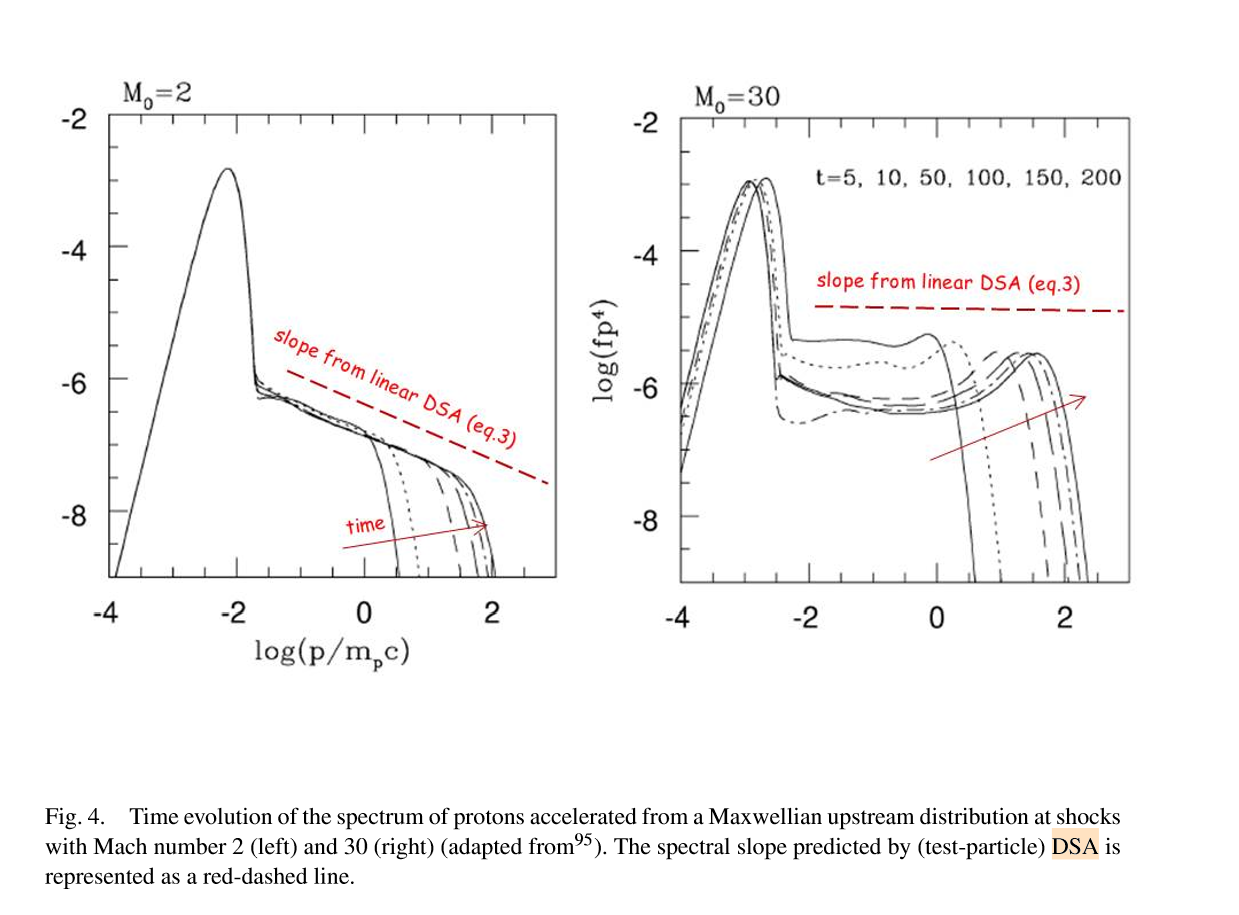
\includegraphics[scale=1]{DSA.png}
\end{figure}
 
\section{Structure Formation Shock Waves}
The flows of the cosmological large-scale structure formation are predicted to produce frequently \tbf{shock waves at the boundaries of clusters and filaments} of galaxies and \tbf{during cluster merger}. 
\begin{\cbox}
 A radio polarization of $27\%$ was detected from the radio relic (Giovannini et al., 1991), but not from the tails of NGC 4789 feeding the relic with radio plasma. This is a clear signature of the \textbf{alignment of magnetic fields enhanced in the shock compression}. The polarization vectors are consistent with a shock wave oriented parallel to the main axis of the radio relic (Enslin et al., 1998). This helps with our case of shocks re-energising the fossil plasma.
\end{\cbox}
\section{Fossil Radio Plasma}
\textbf{Section to be read later}
\section{The Formalism}
Let 'p' be the dimensionless momentum of an ultra relativistic electrons defined as $p\equiv \frac{P}{m_e c}$. This momentum changes as a result of 
\begin{itemize}
\item \tbf{synchrotron losses} proportional to the magnetic energy density $u_B$
\item \tbf{inverse Compton (IC)} losses proportional to the CMB field energy density $u_C$
\item \tbf{adiabatic losses or gains} connected to the change of the volume V of the radio plasma
\end{itemize}
The temporal variation of momentum is  given by the relation
\begin{equation}\label{eqp}
-\de{p}{t}=a_0(u_B+u_C)p^2 +\frac{1}{3}\frac{1}{V}\de{V}{t}p
\end{equation}
Here $a_0=\frac{4}{3}\sigma_T/(m_ec)$. The First term on right side represents sum of magnetic energy density and cosmic energy density while second term represents adiabatic energy loss or gained\\

\tbf{Q. Are there any other losses to consider of?}\\
\tit{We, do not consider bremsstrahlung and Coulomb losses because of very low particle density within Radio plasma}.\fn{What are coulomb losses? is it some analogy to $I^2R$ loss.}\\

Sufficient pitch angle scattering is considered to keep the electron pitch angle distribution isotropic which is with regards to JP model. Electron pitch angle is basically the angle between velocity vector of electron and the magnetic field. \\

The compression ratio is defined as:
\begin{equation}
C(t)=\frac{V_0}{V(t)}
\end{equation}
If C is greater than 1, then gas is compressed with respect to its initial state.\\

Let us try integrating \eqref{eqp} by first allowing a change of variables form $p(t)\rightarrow \tilde{p}(t)=C(t)^{-1/3}p(t)$.\\

\tbf{*Do the integration later*}

\begin{eqnarray*}
-C(t)^{-1/3} \cdot \de{p}{t}=C(t)^{-1/3} \cdot a_0(u_B+u_C)p^2 +C(t)^{-1/3} \cdot \frac{1}{3}\frac{1}{V}\de{V}{t}p\\
\implies -\cc{\frac{V(t)}{V_0}}^{1/3} \cdot \de{p}{t}=\cc{\frac{V(t)}{V_0}}^{1/3} \cdot a_0(u_B+u_C)p^2 + \cc{\frac{V(t)}{V_0}}^{1/3}\cdot \frac{1}{3}\frac{1}{V}\de{V}{t}p\\
\implies - \cc{V(t)^{1/3}} \cdot \de{p}{t}=\cc{V(t)}^{1/3} \cdot a_0(u_B+u_C)p^2 +  \frac{1}{3}\frac{1}{V^{2/3}}\de{V}{t}p\\
\end{eqnarray*}

The result being
\begin{equation}\label{eqp2}
p(p_0,t)=\frac{p_0}{C(t)^{-1/3}+\frac{p_0}{p_\star (t)}}
\end{equation}
\tit{Note that instantaneous momentum is dependent on two quantities, the compression rate which is determined by the environment of the radio cocoon and the $p_\star$ which depends on the energy densities of losses from the cocoon.}\\

and $p_\star$ is defined as \tbf{Characteristic Momentum}. This is basically the momentum only due to energy losses in Synchrotron and compton effect for rate of change of volume to be zero.

\begin{equation}\label{eqpstar}
\frac{1}{p_\star(t)}=a_0\int^t _{t_0} dt^\prime \cc{u_B(t^\prime)+u_C(t^\prime)}\cc{\frac{C(t^\prime)}{C(t)}}^{1/3}
\end{equation}


Now, from \eqref{eqp2} it is clear that for increase in energy density in fields and hence higher losses, the momentum would be governed by compression ration. Higher compression, higher momentum.\\


Now suppose, the change in volume was approximated as,\tit{power law in time}
\begin{equation}
V(t)=V_0\cc{\frac{t}{t_0}}^{b}\;\;\text{ or }\;\;C(t)=\cc{\frac{t}{t_0}}^{-b}
\end{equation}
\tbf{Q. What gives us the precedent of formalizing the variation of volume to a dominant single power of time and how wrong we can be if it is more of an expansion form?}\\

Therefore as time passes for a positive value of 'b', the compression ratio of gas decreases, i.e. gas is expanding with respect to time. Now, this power law will help to provide an analytic solution to \eqref{eqp} \tbf{Find this analytic solution!!!!}\\

\begin{\cbox}
As a further assumption, the photon energy density is considered to be constant, \tit{as our theory is dominated by CMB background radiation, } it does not change with timescales considered here.\\
\end{\cbox}
Further we assume, the magnetic field energy density scales as
\begin{equation}
u_B(t)=u_{B,0}(V/V_0)^{-4/3}=u_{B,0}(t/t_0)^{-4b/3}
\end{equation}
\tbf{as one would expects for an isotropic expansion of the magnetized plasma-- Look into Ruta's thesis and Longair's High energy astrophysics eq. 11.8!!!}\\


The above assumptions help us to integrate \eqref{eqpstar}. We will in addition to above assumptions also exclude the case of $b=3$ and $b=3/5$ (as they give logarithmic relations instead of power laws).[\tbf{we are yet to derive all results and even see why values of b is refuted}].\\

So, we have the \tbf{characteristic momentum of electron} defined as 
\begin{equation}
p_\star(t)=\frac{C^{1/3}}{a_0t\cc{\frac{C^{5/3}-C^{1/b}}{1-5b/3} u_{B,0}+\frac{C^{1/3}-C^{1/b}}{1-b/3} u_{C,0}}}
\end{equation}
\tit{We can see from the above equation why those values of b where refuted- the above expression of $p_\star$ would blow up.}\\


\tbf{\tit{Here, $C=C(t)$ for brevity}}. \\

The the synchrotron and Inverse Compton - cooling produces a sharp upper cut off in the electron distribution$f(p,t)$ at $p_\star(t)$, \tbf{even if the original distribution $f_0(p_0)$ at time $t_0$ extended to infinity. That would mean the at a time t once we go beyond $p_\star$ the electron distribution would fall very sharp}.\\

The electron density per volume and momentum $f(p,t)dpdV$ for $p<p_\star(t)$ \fn{is it because, $p=p_\star$ is the cut-off, and we expect approximately all of electrons to have a momentum less than the characteristic momentum?} is given by
\begin{equation}\label{eqedis}
f(p,t)=f_0(p_0(p,t))\pe{p_0(p,t)}{p}C(t)
\end{equation}
where 
\begin{equation}\label{eqpdis}
p_0(p,t)=\frac{pC(t)^{-1/3}}{1-p/p_\star(t)}
\end{equation}
Now, if the original distribution was a power law
\begin{equation}\label{eqe0dis}
f_0(p_0)=\tilde{f_0}p^{-\alpha_e} _0
\end{equation}
for $p_{min0}<p_{0}<p_{max0}$\fn{Here, we do not want to consider electrons which do not have enough momentum to emit significant synchrotron and hence we have set $p_{min0}$ }, the resulting spectrum is 
\begin{equation}\label{eqetdis}
f(p,t)=\tilde{f_0}C(t)^{\frac{\alpha_e +2}{3}} p^{-\alpha_e}\cc{1-p/p_\star(t)}^{\alpha_e-2}
\end{equation}
for $p_{min}(t)=p(p_{min0,t})<p<p_{max}(t)=p(p_{max0,t})$. In order to obtan \eqref{eqetdis} we just need to substitute \eqref{eqe0dis} and \eqref{eqpdis} in \eqref{eqedis} \\

\tit{\tbf{N.P.:}existence of synchrotron cutoff means the that radiation pattern is not entirely synchrotron and hence  the cut off would represent the frequency after which the radiation pattern is no longer the same synchrotron of spectral index $\alpha_e$ }

\tbf{We are interested in the situation where several phases of cooling characterized by different expansion or contraction rates and durations shaped the electron distribution as the time progressed. Note with require both rates of expansion and duration of phases to accomplish the task of formulation. Both are not the same.}\\

 We write $ p_1 = p(t_1)$ for the \tbf{momentum of an electron originally at $p_0$ after phase 1}. The $p_1$ is characterized by
\begin{itemize}
\item the compression during this phase $C_{0 1} = C(t_1)$
\item and $p_{\star 0 1} = p_\star(t1)$
\end{itemize} 
   \tbf{$p_2=p(t_2)$ for the momentum of the same electron after phase 2, characterized by $C_{1 2}=C(t_2)$ and $p_{\star1 2}=p_\star(t2)$, and so on.}\\
 It is straightforward to show that, the final electron momentum(\tbf{momentum of same electron after n stages, calculated directly after n stages after stage 0}) $p_n$ after n such phases can still be written in the form
 \begin{equation}
 p_n(p_0)=\frac{p_0}{(C_{0n})^{-1/3}+p_0/p_{\star 0n}}
 \end{equation}
 where 
 \begin{equation}
 C_{0n}=\Pi_{i=1} ^nC_{i-1i}=\Pi^n _{i=1}\frac{V_i-1}{V_i}=\frac{V_0}{V_n}
 \end{equation}
which is basically the compression ratio of the final and initial configuration and maximal final momentum is given by
\begin{equation}
\frac{1}{p_{\star 0n}}=\sum^n _{i=1}\frac{(C_{0i-1})^{1/3}}{p_{\star i-1 i}}
\end{equation}
The effects of the individual cooling phases sum up weighted by $(C_{0 i}) ^{1/3}$ . Thus, \textbf{whenever the radio plasma is most extended, cooling is inefficient}\\
It remains to provide the parameters describing the different phases.\\ \tbf{Now, suppose we want to describe a phase i where the expansion or compression is described by $b_i$, and two of the following three quantities are given: $\tau_i$, the time scale of expansion, $C_{i-1i}$, the compression ratio during the phase, and $\Delta ti$, the duration of the phase. These quantities are related via }
\begin{equation}\label{eqCi}
C_{i-1i}=(1+\Delta t_i/\tau_i)^{-b_i}
\end{equation}
We get
\begin{equation}\label{eqpdisi}
p_{\star i-1i}=\frac{C^{1/3}}{a_0t_i\cc{\frac{C^{5/3}-C^{1/b}}{1-5b/3} u_{B,i-1}+\frac{C^{1/3}-C^{1/b}}{1-b/3} u_{C}}}
\end{equation}
where, $C=C_{i-1,i}$ and $t_i=\tau_i+\Delta t_i$\\
The magnetic energy density at the beginning of the phase i is that of the end of the phase, phase $i-1$:
\begin{equation}
u_{B,i-1}=u_{B,0}(C_{0,i-1})^{4/3}
\end{equation}
The resulting electron spectrum from an initial power law distribution is 
\begin{equation}
f_i(p)=\tilde{f_0}C^{\frac{\alpha_e+2}{3}}_{0i} p^{-\alpha_e}(1-p/p_{\star,0i})^{\alpha_e-2}
\end{equation}
for $p_{min\;\;i}(t)=p_i(p_{min0})<p<p_{max\;\;i}(t)=p_i(p_{max0})$ and $f_i(p)=0$ otherwise.\\
The synchrotron emission at a given frequency is 
\begin{equation}
L_{\nu\;\;i}=c_3B_i V_i \int^{p_{max\;i}} _{p_{min \; i}} dpf_i(p) \tilde{F}(\nu/\nu_i(p))
\end{equation}
where $c_3=\sqrt{3}e^3/(4 \pi m_e c^2)$ and the characteristic frequency $\nu_i(p)=3eB_ip^2/(4 \pi m_e c)$. The dimensionless spectral emissivity of a mono-energetic isotropic electron distribution in isotropically oriented magnetic fields $\tilde{F}(x)$ can be approximated :
\begin{equation}
\tilde{F}(x)\approx \frac{2^{2/3}(\pi/3)^{3/2}}{\Gamma(11/6)}x^{1/3}\exp\cc{\frac{-11}{8}x^{7/8}}
\end{equation}
In reality, after shock passage an originally isotropic ensemble of field lines gets partially aligned with the shock plane. This is also true for the unshocked radio plasma, since its morphology gets significantly flattened during compression (see phase 3 in Sec. 5). This would produce a radio polarization and a luminosity which depends on the viewing angle (Enslin et al., 1998). As long as we are only calculating the total luminosity of the radio cocoon/relic,this can be ignored. But, in case one wants to know the expected flux, one has to correct for the anisotropic emission pattern of the cluster radio relics. Fortunately, the degree of radio polarization can be used to determine the viewing angle with respect to the shock plane (Laing, 1980; Enslin et al., 1998).\\
The upper cutoff in the electron distribution at $p_{\star \;\; 0 \; \;n}$ produces a cutoff in the synchrotron spectrum near $\nu_{\star n} = \nu_c(p_{\star 0n})$. But since $\tilde{F}(x)$  has a broad maximum even a sharp cutoff in the electron spectrum gives a soft cutoff in the radio, with significant flux above $\nu_{\star n}$.

\section{The Model}
The radio plasma goes various stages of expansion and contraction between the release of the matter from radio galaxy and the reappearance as cluster radio relic:
\begin{itemize}
\item \tbf{Phase 0: Injection}
\begin{itemize}
\item The radio galaxy is active and a large expanding volume is being filled with radio plasma.
\item assuming that there is no gas density gradient in the vicinity of the radio galaxy, The expansion of this cocoon is likely to be supersonic (with respect to the outer medium) and therefore $b_0 = 9/5$ \tbf{(Kaiser and Alexander, 1997)}.\tbf{How did we get the value of $b_0$}
\item the typical age of a radio source at the end of nuclear activity (Alexander and Leahy, 1987, for typical ages) is around $\tau=0.15 Gyr$. We assume that the injection occurred with the same time constant.
\item by injection of fresh electrons, The particle population is kept close to a power-law distribution. In flux vs frequency plot, we assume a  spectral index of $\alpha_e = 2.5$ and an upper cutoff at $p_{max0} = 10^5$. The momentum cut-off produces a radio cut-off above $42GHz(B/\mu G)$.\tit{The results are not very sensitive to the choice of this parameter.} \tbf{ More realistic electron spectra at the end of phase 0 could be constructed by superimposing the spectra of the electron populations of different ages}, as in the models of Kaiser et al. (1997). \tit{But, for the present purpose of demonstrating that \tbf{the fossil radio plasma can be revived by compression}, our simplified treatment should be sufficiently illustrative. }\tbf{Look into the sources to get all the parameters correct!!}
\end{itemize}
\item \tbf{Phase 1:Expansion}
\begin{itemize}
\item Once the central engine of the radio galaxy became inactive, the radio cocoon might still be strongly over-pressured compared to its gaseous environment (Begelman and Cioffi, 1989). \textbf{This is because of the internal pressure of plasma on the cocoon surface?}\tit{ So does a surface actually exist which we call cocoon, that prevents diffusion of plasm into the surrounding medium?}
\item  If this is the case a Sedov-like expansion phase exists with $b_1 = 6/5$. \tbf{The answer to my previous question lie in sedov like expansion phase}
\item Momentum conservation of the expanding shell around the cocoon forces the expansion rates at the end of phase 0 and beginning of phase 1 to be the same, leading to $\tau_1 = \frac{b_1}{b_0} \tau_0 = \frac{2}{3}\tau_0$. 
\item \tbf{ The expansion will significantly deviate from $b_1 = 6/5$ at the moment when the \tit{internal pressure drops to a value comparable to the environmental pressure}.}
\item We simplify this behaviour by assuming that \tbf{the expansion is Sedov-like until pressure equilibrium} is reached. The \tbf{radio cocoon probably becomes undetectable} during this phase, and therefore becomes a fossil radio cocoon or a so called \tbf{radio ghost}.
\end{itemize}
\item \tbf{Phase 2: Lurking.}
\begin{itemize}
\item In this phase the Pressure equilibrium with the environment is reached, and the volume of the radio plasma remains more or less constant. Therefore, in this stage, $C_{12}\approx 1$ and $b\approx 0$. Now, we consider this phase to last very long time and hence we consider $\tau_2 \rightarrow \infty$ in \eqref{eqpdisi} to get 
\begin{equation}\label{eqp12}
p_{\star 12}=\rr{a_0(u_{B2}+u_{C}\Delta t_2)}^{-1}
\end{equation}

\item Due to the \tbf{previous adiabatic energy losses} of the electrons, they reside at \tbf{low energies during phase 2}.\tit{Are adiabatic losses a part of sedov expansion phase?}.
\item Their radiation losses, which strongly depend on the particle energies, are therefore strongly diminished.  Additionally, the synchrotron losses are further reduced due to the weaker magnetic field during the expanded state of the radio cocoon.
\item The adiabatic losses are reversible, and will be reversed during the subsequent compression phase, whereas the radiative losses are irreversible. Since \tbf{the latter are suppressed during this phase}, the radio ghost state can be called the \tbf{energy saving mode of a radio cocoon.}
\end{itemize}
\item \textbf{Phase 3: Flashing:} 
\begin{itemize}
\item At this stage The fossil radio plasma gets dragged into a shock wave of cosmic large-scale structure formation, e.g. at the boundary of a cluster of galaxies or in a galaxy cluster merger event.
\item  While its thermal environment gets shocked, the radio plasma is not shocked due to the much higher internal sound speed.
\item The plasma is only compressed adiabatically because of the shocked external environment . \tbf{The electron population and the magnetic field gain energy adiabatically}, leading to a \tbf{steep enhancement of the synchrotron emissivity.}
\item The duration of this phase is given by
\begin{equation}
\Delta t_3= \frac{V^{1/3}_2}{v_{shock2}}\approx \frac{0.1-1Mpc}{300-3000km/s}\approx \cc{30Myr-3Gyr}
\end{equation} 
where $v_{shock2}$ is the pre shock flow velocity in the shock frame.
\item This preshock flow velocity $v_{shock2}$ is related to pre shock sound speed as $c_{s2}=\sqrt{\gamma P_2/\cc{n_e(m_p+m_e)/2}}$ via
\begin{equation}
v^2 _{shock2}=\frac{c^2_{s2}}{2 \gamma}\cc{\gamma-1+(\gamma-1)\frac{P_3}{P_2}}
\end{equation}
\textbf{Check Landau and Lifshitz 1966} paper, here $\gamma=\frac{5}{3}$ is the adiabatic index of the thermal gas.
\item  The compression factor of the relativistic plasma is high, and can be calculated from the assumed pressure jump $P_3/P_2$ of the surrounding thermal gas, assuming pressure equilibrium before and after the shock passage:
\begin{equation}
C_{23}=\cc{P_3/P_2}^{3/4}
\end{equation}
\item Now we tru to get a rough picture of the compression process, this will also help us achieve the values of $b_3$ and $\tau_3$
\begin{itemize}
\item The sound speed within the radio plasma should be much higher than even in the post-shock thermal environment, (it could be up to $c/\sqrt{3}$, if the plasma is fully relativistic), so that an \tbf{instantaneous response to environmental changes can be assumed.}
\item \tbf{During the shock passage, the cocoon is exposed to the high thermal pressure of the post-shock gas on its down- and to the ram-pressure of the pre-shock gas on its up-stream side.}
\item   But, on the remaining surface the cocoon is only subject to the (much lower) up-stream gas pressure.
\item  The relativistic plasma will therefore start to expand orthogonal to the gas flow, producing a flattened pancake-like morphology. 
\item In order be able to expel the ambient gas sideways \tbf{why would the gas want to do that?} additional internal pressure  comparable to the ram pressure of the expelled material is needed. This pressure is produced by compression. 
\item For that, The process of flattening stops when the ram pressure of the swept-up material at the expanding edges of the pancake is of the order of the ram pressure of the incoming flow \textbf{What is the incoming flow here?}.
\item This implies that the ratio of the diameter to the thickness of the expanded cocoon is roughly 4 for a strong shock.
\end{itemize}
\end{itemize}
  The compression is slow in the beginning, and rapid towards the end when the cocoon is significantly flattened. We mimic this by setting $b_3 = 2$ and a negative $\tau_3$, according to \eqref{eqCi}. We favour this over the more intuitive choice of a positive $\tau_3$ and large negative $b_3$, since \tbf{it describes the process of compression more realistically. }
\item \tbf{Phase 4:Fading}
In this stage,The radio plasma is in pressure equilibrium with the post-shock medium, which should provide roughly a uniform environment: $b_4 = 0$. \tbf{The radio emission of the relic now fades away due to the heavy radiation losses.}

\end{itemize}
\section{The Scenarios}
Here we discuss three different plausible cases and try to illustrate the resulting plausible situations.\\
The following scenarios have been chosen:
\begin{enumerate}
\item \tbf{Scenario A:} In this scenario, the relic is located at the \tbf{center of a galaxy cluster}
\item \tbf{Scenario B:} In this scenario, The location of the relic is near the cluster boundary, i.e., in the \tbf{proximity of the accretion shock wave}.
\begin{\cbox}
In the above scenarios A and B the duration of phase 2 was chosen to be so long that the shocked radio plasma could be barely observed as a weak ultra-steep spectrum source.\\
Additionally, In both the scenarios\\
We assume the initial cocoon (at the end of phase 0) to comtain the magnetic fields and the relativistic particles (electrons and protons)  with energies of $E_{B/e/p}=10^{60}erg$ each. 
\end{\cbox}
\item \tbf{Scenario C:} In this scenario, the phase 2 is chosen shorter as it would henceforth result in moderately steepened spectrum of the cluster radio relic. In this scenario the relativistic energies are assumed to be $E_{B/e/p}=10^{58}erg$
\end{enumerate}
In all the above scenarios,
\begin{itemize}
\item the \tbf{three components produce a \tit{relativistic isotropic pressure of }}:
\begin{equation}\label{eqisoP}
P_{cocoon0}=\frac{E_e+E_p+E_B}{3V_0}
\end{equation}
 \item The spectral index of $\alpha_e=2.5$ and a rather high cut off in the electron spectrum at $p_{max0}=10^5$.(\tbf{This is claimed to have no physical influence on the conclusion.})
 \item The lower cut off in electron spectrum is set at $p_{min0}=10$ in \tbf{scenarios A and B} and $p_{min0}=100$ in \tbf{Scenario C} .\tbf{ The lower cutoffs only affect the normalizations of the radio fluxes, not the spectral shapes. }
\end{itemize}
Now we look at scenarios individually:
\begin{itemize}
\item {Scenario A: The Cocoon at cluster center:}
The pre-cluster merger configuration at the location of radio galaxy are:

\begin{itemize}
\item Electron Density: $n_E: 0.3 \cdot 10^{-3}cm^{-3}$
\item Temperature: $kT=3KeV$
\item Due to high environmental pressure , the internal pressure is assumed only twice of external pressure
\item The initial volume $V_0$ is obtained from \eqref{eqisoP} 
\end{itemize}
Now the following assumptions and processes go in at various stages according accepted phenomenological logic:
\begin{itemize}

 
\item For the revived fossil cocoon to emit within observable frequency range, \tbf{phase 2 cannot last longer than $\Delta t_2=0.1Gyr$}.\\

 \tbf{I want to be able to do these calculations at the end.}
 
\item We assume that the shock wave of a cluster merger event \tbf{increases the internal pressure by $P_3/P_2 = 12$ during the phase 3}. This corresponds to a \tbf{moderate shock with shock compression factor of 2.8}, whereas strong non-relativistic shocks can have a compression factor of 4. \tbf{A moderate shock is expected, since both merging clusters are expected to have temperatures of several keV and therefore sound velocities comparable to the merger velocity.}
\begin{figure}[h!]\label{figsceA}
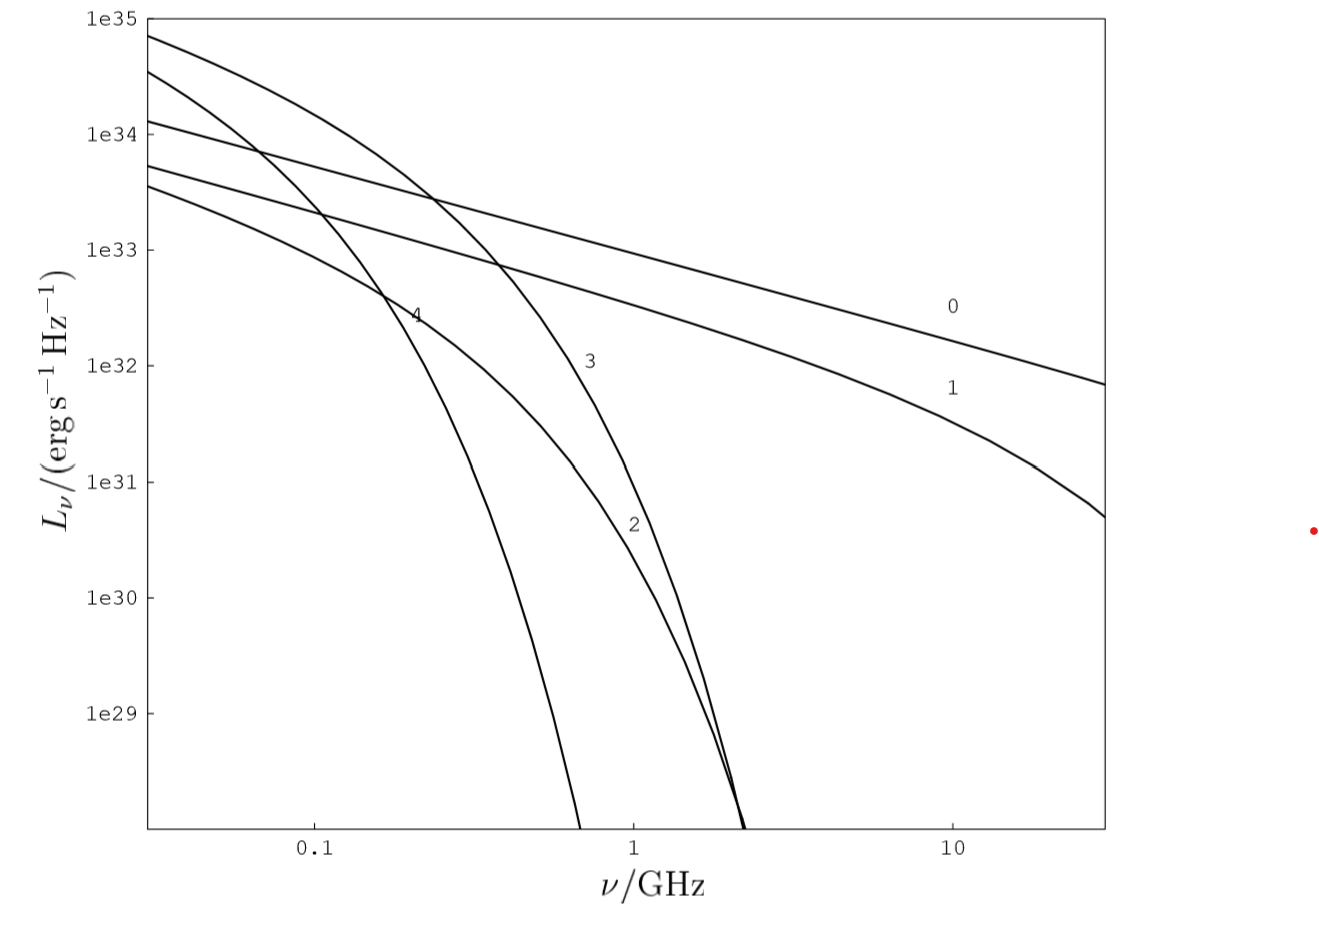
\includegraphics[scale=0.7]{figsceA.png}
\caption{Radio spectrum of the radio cocoon in scenario A at the end of phases 0-4.}
\end{figure}
Check out Figure \ref{figsceA}:
\begin{\cbox}
the compression caused by the merger shock wave gives rise to a burst of low frequency emission, but practically no high frequency emission. This is due to the rapid decay of the upper end of the electron spectrum during phase 3, which essentially wipes out the adiabatic energy gains of these electrons. The source decays on a time-scale of a few tens of Myr, mostly due to the heavy synchrotron losses. If the radio cocoon is located in a more peripheral region of the cluster, where the density, the pressure and therefore the magnetic field strength inside the cocoon is much lower, these losses are also much milder. This lengthens the time scale over which the radiatively cooling synchrotron plasma can still be revived by the next passing shock, and thus rendered radio detectable. We, therefore, expect the radio relic phenomena to be found preferentially at larger cluster radii, and less often near the cluster center (although projection can help some relics to appear near the cluster core). The best environment to find cluster radio relics is, therefore, near the edges of the clusters. 
\end{\cbox}
\end{itemize}
\item \tbf{Scenario B: The Cocoon at the Cluster Boundary}
The radio cocoon is assumed here to be born outside the cluster, in an environment of a dense galaxy filament, or a group of galaxies.\\
The pre-cluster merger configuration at the location of radio galaxy are(the parameters are much lower than the parameters when the cocoon was located at center of the cluster):
\begin{itemize}
\item Electron Density: $n_e=0.3 \cdot 10^{-5}cm^{-3}$
\item Temperature:$kT=0.3KeV$
\item The freshly injected radio plasma might be overpressured by a factor of 100, leading to a short expansion phase(Phase 1). \tbf{This is because the environmental pressure is not high}
\end{itemize} 
The phenomological processes occurring during various stages
\begin{itemize}
\item After this, the electrons within the expanded Mpc sized cocoon suffer mostly the IC-losses, allowing revival of the radio plasma even $\Delta t_2 = 1Gyr$ later .\tit{The revival age for Scenario A cannot be pushed beyond $\Delta t_2=0.1 Gyr$ for Scenario A}. The reason Scenario B has higher revival period is because of very low magnetic fields causing very low synchrotron losses.
\item  The revival can happen when the cocoon along with the ambient medium is crossed by the accretion shock of a cluster of galaxies in the Phase 3, which might entail a pressure jump as large as $P_3/P_2 = 100$, in order to heat the infalling cool gas to the cluster virial temperature of up to 10keV. \tit{For scenario A this was the pressure ratios between phase 3 and phase 2 was 12}
\end{itemize} 
\begin{figure}[h!]\label{figsceB}
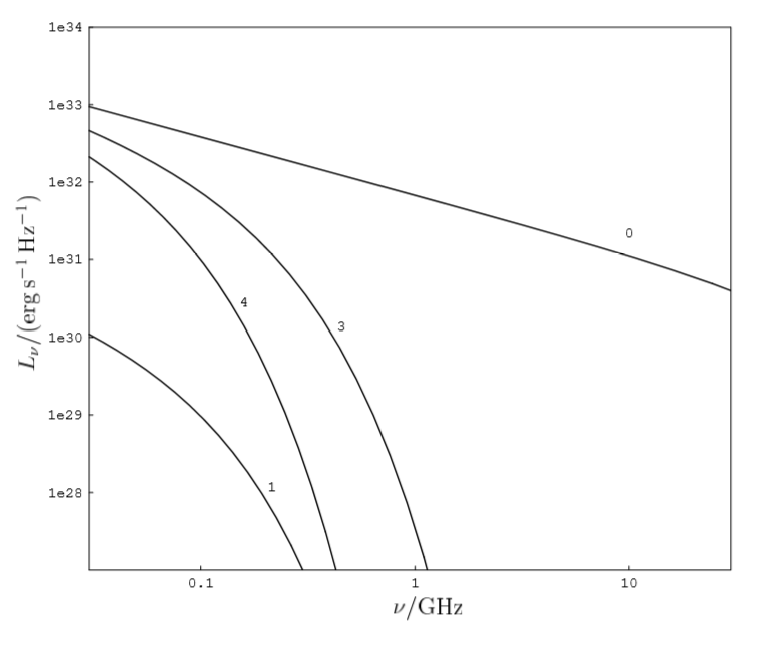
\includegraphics[scale=0.75]{figsceB.png}
\caption{Radio spectrum of the radio cocoon in scenario B at the end of phases 0-4.  The luminosity at the end of phase 2 is too small in order to be displayed in this figure.}
\end{figure}
Check out Figure \ref{figsceB}
\begin{\cbox}
Scenario B can explain the steep and bent radio spectrum of the cluster radio relic 0038-096 in Abell 85. An eye-fit to the radio spectrum (Fig. 5) shows that the maximal electron momentum in this case is $p_\star = 10^4 (B/\mu G)^{-1/2}$. The magnetic field strength of the cluster relic was estimated from the minimum energy argument to be $B \approx 1\mu G$ (Feretti and Giovannini, 1996) and from the detection of excess X-ray emission at the location of the relic, which implies a field strength of $B = 0.95 \pm 0.10\mu G$ (Bagchi et al., 1998) if this emission refers to the IC scattered cosmic microwave background photons, otherwise a higher field strength. Using $B = 1\mu G$ and $p_\star = 10^4$ and assuming a uniform environment without expansion and compression, an age of 0.2Gyr would result (Komissarov and Gubanov, 1994, and see Eq. \eqref{eqp12}). But scenario B demonstrates that the radio plasma can be as old as 2Gyr. This resolves the problem of the apparent cooling time of the electrons being too short for any nearby galaxy to have ejected the plasma and then moved to its present location with a typical velocity of a cluster member. For the long duration of phase 2 the resulting spectrum is fairly steep in the observable radio range. But this need not to be the case for a scenario with a shorter fossil phase. 
\end{\cbox}
\item \textbf{Scenario C: The Smoking Gun}
 In order to substantiate the last statement, we choose a set of parameters for scenario C which produces a cluster radio relic with relative flat, nearly unbent radio spectrum.\\
 The characteristics of the cocoon pre-cluster merger are
 \begin{itemize}
 \item electron density $n_e=0.3 \times 10{-5}cm^{-3}$\\
 \item $kT=0.6KeV$
\end{itemize}  
 The inflow of the plasma and the compression at the cluster accretion shock wave might have taken a few hundreds of Myr. We assume a pressure jump of only $P_3/P_2 = 40$ at the shock wave, not higher, in order to allow the temperature of the post-shock gas to stay below the average cluster temperature of 8.2KeV  As can be seen in Fig. \ref{figsceC}, the radio spectrum below 1 GHz stays practically unbent for a couple of tens of Myr after the shock passage.
\begin{figure}[h!]\label{figsceC}
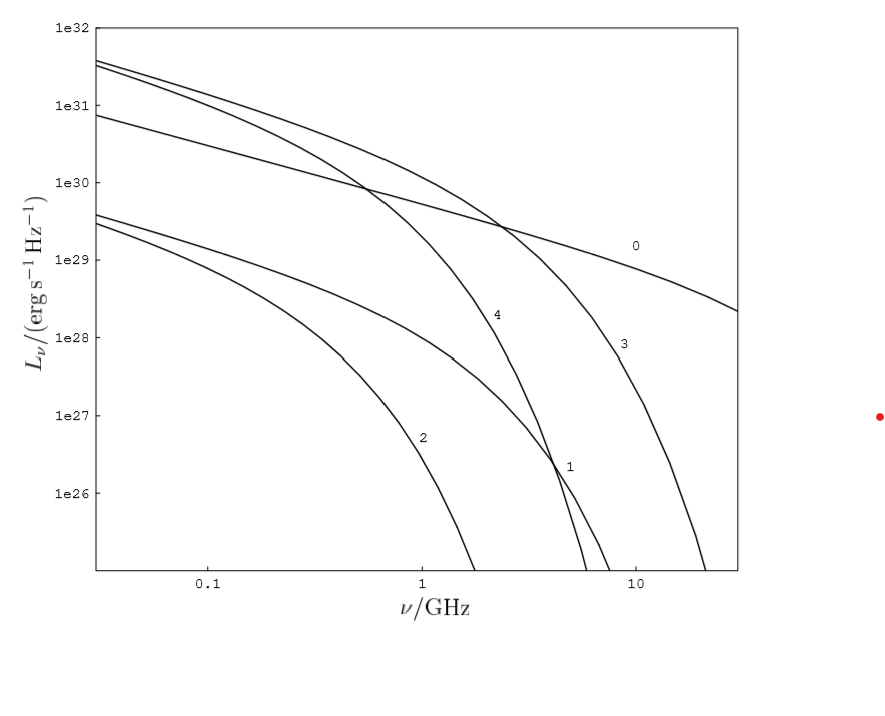
\includegraphics[scale=1]{figsceC.png}
\caption{Radio spectrum of the radio cocoon in scenario C at the end of phases 0-4.  }
\end{figure}
\end{itemize}
\chapter{Cocoons Of Radio Galaxies}
\tbf{This section is taken up from Intergalactic Matter And Cocoons of Radio Galaxies by \tit{Biman B. Nath}}. Refer \tit{Begelman and Cioffi for more details,1989. Overpressured Cocoons in Extragalactic Radio sources}\\
\tbf{What are radio cocoons?}\\
A cocoon is a natural by-product of the propagation of a supersonic jet through a denser ambient medium. Given a high-pressure jet, the slow lateral expansion of the cocoon guarantees that the average cocoon pressure will exceed the ambient pressure in the initial stages of the jet evolution. 

\tbf{What keeps the cocoons expanding?}
Cocoons have been shown to remain overpressured with respect to the ambient medium for most of their lifetime of the source.\\


 It has long been evident that supersonic, low-density jets deposit most of their energy in the cocoon, which acts as a "wastebasket" (\tit{Scheuer, P. A. G. 1974, MNRAS, 166, 513.
}).\\

\tbf{Where does the idea of overpressure come into picture?}\\
Recently, however, Begelman and Cioffi ( \tit{Begelman, M. C., and Cioffi, D. F. 1989, ApJ, 345, L21}; hereafter BC) argued that the cocoons remain overpressured with respect to the ambient medium for a long time, and that for many sources, they have not yet reached a state of equilibrium. They then used this fact to address the problem of jet confinement by the ram pressure of the cocoon.

\tbf{So, what is the intutive picture we have of cocoons?}\\
\begin{\cbox} 
The picture that emerges from these studies is that of a overpressured, jet-nourished cocoon, whose length and width depend on the balance of the ram pressure of the ambient medium with, respectively, the jet's momentum flux and the cocoon pressure. 
\end{\cbox}

Here we use, the value of hubble constant as $H=h_{50}\;\;km\;\;s^{-1}\;\;Mpc^{-1}$.
\section{Overpressured Cocoons}
\tbf{Why the jets produced cocoons must be light and hypersonic?}\\

We will not consider heavy jets to form cocoons as  Heavy jets behave like 'bullets' and do not form cocoons. And since the jet luminosity is proportional to$ M^3_h$ (M is the Mach number of the head of the jet with respect to the sound velocity of the ambient medium), high luminosity of the classical double jet implies hypersonic, if not supersonic, jets.\\

Now, here we have assumed the $\rho_j$ is smaller that of the ambient medium $\rho_a$ i.e. $\eta=\rho_j/\rho_a$. \\

\tbf{Mechanics of cocoons:}\\

Let us assume that $L_j$ be the jet power which is constant in time for simplicity.\\

\tbf{Finding velocity of jet data:}\\

The velocity of the head of the jet $v_h$ is determined by the balance of the thrust of the jet($\sim L_j/v_j$) spread over the cross sectional area $A_h$ of the bow shock at the end of the jet and the ram pressure of the ambient medium. This yields
\begin{equation}
v_h \sim \cc{\frac{L_j}{\rho_a v^3_j A_h}}^{1/2}v_j
\end{equation}
Notice that $A_h$ can be much larger than the cross-section of the jet itself. The cocoon pressure is given by dividing the total energy deposited by the jet inside the volume of the cocoon $V_c= \epsilon_V (2\pi r^2_c)l_h$ where $r_c$ is half width of the cocoon at the center , $l_h=\int v_h dt$ is the length of the jet head and $\epsilon_V$ is the volume factor depending on the shape of the cocoon. The value of $\epsilon_V$ is
\begin{itemize}
\item 1 for cyclindrical cocoon
\item 1/3 for biconical
\end{itemize} 
One thus obtains 
\begin{equation}
p_C=\frac{(\gamma-1)L_jt}{V_c}\approx \rho_A\cc{\de{r_C}{t}}^2
\end{equation}
Here the second equality comes from balancing the cocoon pressure with the ram pressure of the ambient medium. $\gamma$ is the adiabatic index of the material in the cocoon. This readily yields upon integration an expression for the size of the cocoon as:
\begin{equation}
r_c^2 \approx \cc{\frac{6 (\gamma -1)}{\pi}}^{1/2} \cc{\frac{L_jv_jA_h}{\rho_A}}^{1/2}\cc{\frac{\epsilon_V}{1/3}}^{-1/2}t^{-1}
\end{equation}
And the above two equations can be combined to give the cocoon pressure, as
\begin{equation}
p_c\approx \cc{\frac{9(\gamma-1)}{24\pi}}^{1/2}\cc{\frac{L_j \rho_a}{v_h}}\cc{\frac{\epsilon_V}{1/3}}^{-1/2}t^{-1}
\end{equation}
The last equation  allows us to estimate the time $t_{eq}$ for the cocoon to reach pressure equilibrium with the ambient medium, after which the cocoon boundary expands at the sound speed of the ambient medium. For powerful radio galaxies, with length-scales of the order of Mpc, the ambient medium is the IGM. We can write the equilibrium time
scale as,
\begin{eqnarray}
t_{eq}\approx\frac{\mu m_p}{kT_a}\cc{\frac{L_jv_jA_h}{\rho_a}}^{1/4}\cc{\frac{9(\gamma-1)}{24 \pi}}^{1/2}\cc{\frac{\epsilon_V}{1/3}}^{-1/2}\\
\sim 1.34 \times 10^{10}(T_{a,6})^{-1}\Omega^{-1/4}_{IGM}h^{1/2}_{50}L^{1/4}_{j,45}\beta^{1/4}_j A^{1/4}_{h,30}\cc{\frac{\epsilon_V}{1/3}}^{-1/2}yr
\end{eqnarray}
Here,
\begin{itemize}
\item $\mu \sim 0.6$ is the molecular weight\\
\item $T_a=10^6 T_{a,6}K$ is the temperature of the IGM gas
\item k is the boltzman constant
\item $L_j$ is in the units of $10^{45}erg\; s^{-1}$ 
\item $A_h$ is in the units of $30kpc^2$
\end{itemize}

\chapter{Ruta Kale's Thesis}
\section{Introduction}
\section{Radio Relics}
Diffuse radio sources with filamentary, elongated morphologies, not associated with any active galactic nucleus are termed as radio relics (e.g. Ferrari et al 2008). \\
\textbf{\tit{may be they are not at all related to merger and they are just related to dead radio galaxies and the reason these dead galaxies get re-accelerated are the merger events}}\\
These can either be associated with galaxy clusters \tbf{(cluster radio relics)} or can be remnants of radio galaxies \tbf{(relic radio galaxies)}.\\
\textbf{\tit{May be cluster radio relics and relic radio galaxies are not different and can be united to form a single group of relics, we can do this if we see similar attributes in structures or if we analyse the outcome of a particular relic radio galaxy being subjected to a shock and if the results are same as cluster radio relics we can have a united front}}.\\
\textbf{Properties of these relics:}
Such sources typically have steep synchrotron spectra ($\alpha$ > 1) and high degree of polarization $(\sim 10\% - 40\%)$ (Ferrari et al 2008 for a recent review). The linear sizes of the relics range from
200 kpc to 2 Mpc. Relics are also low surface brightness ($\sim mJy$ $arcmin^{-2}$ at 1.4 GHz) sources and occur in only $\sim 6\%$ of all clusters (Giovannini et al 1999). \\
\textbf{\tit{it would be great if would be able to predict, which clusters should we observe relics (we, can give a methodology for the same!) and second think on the reason why we don't see relics more often}}
\subsection{Fossil/Relic Radio Galaxies}
Radio galaxies produce jets which pump relativistic plasma into the surrounding medium. Back flows of the relativistic plasma are formed at the end of the jet and the non-thermal plasma(\tbf{\tit{just referring to non-Maxwellian distribution of particles}}) occupies regions surrounding the jets forming lobes.\\
\textbf{What happens to these lobes when the AGN switches off?}
 The overpressured lobes expand, even after the AGN switches off, until pressure equilibrium is attained and form structures like cocoons.\\
\tbf{\tit{here, we are not questioning, whether to form such lobes in lifetime of AGN is feasible at all by the same mechanism? I mean does the current state of relic be related to expanded lobes numerically?}}\\ 
 
 The PdV work done on the surrounding medium during expansion amounts to a loss in energy. \tbf{\tit{I would like to calculate if it is actually that feasible and timescales match!}}\\
 
 Such cocoons can remain detectable after the AGN stops to be active for only about 10-100 million years.
\tbf{\tit{what are the various processes, by which this non thermal plasma,loose energy, a complete description of which will give us a handle on lifetime of such galaxies. It is just hard to relate if it is just synchrotron, then why do we have a number that has a factor of 10 i.e. there age may go from 10 to 100 mil.}} \\
  These can be then seen as filamentary, elongated or double
lobed radio sources with no obvious jets or cores. \\
\textbf{The short lifetimes can be the reason for a rarity of such sources. }For example, the relic in the cluster A85 (Slee
et al 2001) could be such a fossil (Fig. 1.7, left). Other examples of such relics are A133 (Fig. 1.6, right) (Slee et al 2001) and the relic in A4038 (Slee et al 2001; chapter 4).\\
\tit{There have been attempts to model the radio spectra of such sources to extract parameters such as the \tbf{timescale over which the AGN was active, the time spent by the plasma in relic phase and the magnetic field (Komissarov $\&$ Gubanov 1994; Slee et al 2001; Kaiser $\&$ Cotter 2002).} } There are two basic approaches:
\begin{enumerate}
\item \tbf{The JP models(Jaffe and Perola (1973)):}\textbf{ In this approach the pitch angle of the electrons is assumed to isotropize much faster than the energy loss timescale}. Alfvén wave is a type of magneto hydrodynamic wave in which ions oscillate in response to a restoring force provided by an effective tension on the magnetic field lines. The scattering of electrons off the Alfen waves causes the isotropization. \tbf{ The models which use the assumption of isotropization of pitch angles are regarded as JP models.}
\item \tbf{The KP model:}
\end{enumerate}

\section{Chapter 2:}
\section{Summary}
The primary aim of the thesis was to understand
the origins of radio halos and relics in clusters of galaxies. 
\subsection{Results}
\begin{itemize}

\item The multi-frequency (150, 350, and 1369 MHz) analysis of the radio halo and the relic in A2256 indicates that turbulent reacceleration during mergers may be the mechanism that generated the radio halo and the relic. \textbf{\textit{Refer Chapter 2: It would help you understand, how do we point out that a process or a result is indicative of turbulent re-acceleration}}.\\
The flat spectrum NW region of the relic ($\sim$ 200 kpc region, showing polarization upto $45\%$ at 1.4 GHz, CE06) could be the result of the current activity of a shock that passed through the cluster from SE to NW.\textbf{\tit{Shouldn't in order to conclude that a particular relic is a result of shock activity, should we say that the electrons age with time? What about the flat spectrum helps us know if a shock led to origin of particle acceleration}}\\
 The low frequency steepening of the spectra of the diffuse radio emission in A2256 (spectral index maps, Figs. 2.2 and 2.4) is interpreted as the result of superposition of spectra of relativistic electrons accelerated at two epochs. These two epochs are interpreted to be the two mergers that are proposed to have occurred based on X-ray and optical observations (Sun et al 2002; Berrington et al
2003).

\item b

\item c
\item d
\item  The identification of ultra-steep spectrum ($\alpha < - 1.8$) sources from the NVSS and the VLSS and their imaging at 330 MHz (VLA) and at 1.4 GHz (GMRT) led to the discovery of double lobed sources with no obvious presence of cores and jets (AGN).\textbf{\tit{What is NVSS and VLSS?}}\\
 These are interpreted to be dead radio galaxies.\\
\textbf{Can there be other possibilities, can it just be dust clouds and not exactly relics?}\\ 
  The model of lurking radio cocoons implies that most of these are sources which have been in the 'relic' phase (AGN off) for more time than the time scale for which the AGN was active. \\\textbf{Why?}\\
Assuming a mean redshift of 0.2 (4 of the 10 sources are at this redshift) for these sources, the present luminosities ($L_{1.4} \sim 10^{24}W Hz^{-1}$) imply that their luminosities in active phase would have been 10 - 100 times of those of the brightest AGN s in the local universe.\\
\textbf{Do the same calculation, again!}\\

With the detection limits of the VLSS and the NVSS only the brightest among such dead radio sources could be detected. The luminosity function of the currently active AGN indicates that the number density of sources with power $L_{1.4} \sim 10^{24} W Hz^{-1}$ is 100 times higher than with $L_{1.4} \sim 10^{27} W Hz^{-1}$ (Sadler et al 2002) and more sensitive surveys will be able to detect these.\\
\textbf{I don't understand , this point!}\\

 These studies will
lead to the understanding of the various stages of AGN evolution. (Chapter
5; Dwarakanath, K. S. $\&$ Kale, R. 2009, ApJL, 698, 163)


\end{itemize}
\chapter{List Of Sources}
Below I present the list of sources by unifying data from DB1-$www.galaxyclusters.com$ and DB2(Bold font)-$https://arxiv.org/pdf/1808.04057.pdf
$
\begin{itemize}
\item The list is organized in ascending order of Redshift .\\
\item First column indicates designation of source.Second column represents Redshift as provided in DB1  and Third column represents Redshift from DB2.
\end{itemize}

\begin{center}
\begin{tabular}{|c|c|c|c|c|}
\hline 
\tbf{Designation} & Redshift1(z) & Redshift2 & Frequency(MHz) & Surface Brightness(mJy)\\
\hline
\multirow{4}{*}{AS753} & 0.0130 & \tbf{0.014} & 2378 & 100\\
&&&330&8500\\
&&&1398&460\\
&&&843&1300\\
\hline
\multirow{7}{*}{A4038} & 0.0303 & \tbf{0.02819}&843&170$\pm$30\\
&&&80&19000$\pm$2700\\
&&&160&4300$\pm$500\\
&&&327&1440$pm$150\\
&&&1400&61$\pm$3\\
&&&408&910$\pm$110\\
&&&30&32000$\pm$7000\\
\hline
\tbf{A2063}&&\tbf{0.0349}\\
\hline
\tbf{A548b-NW} &&\tbf{0.0424}\\
\hline
\tbf{A548b-N} &&\tbf{0.0424}\\
\hline
\multirow{11}{*}{A85}& 0.0557 & \tbf{0.0551}&843&200$\pm$30\\
&&&16&93000$\pm$24000\\
&&&80&34000$\pm$3700\\
&&&2700&10\\
&&&300&2739\\
&&&1400&43$\pm$3\\
&&&30&93000$\pm$13000\\
&&&408&1540$\pm$250\\
&&&1425&40$\pm$2.3\\
&&&160&8330$\pm$700\\
&&&327&3200$\pm$320\\
\hline
\multirow{11}{*}{A133} & 0.0603&&4900&4$\pm$0.3\\
&&&2700&29$\pm$16\\
&&&1400&168$\pm$6\\
&&&843&530$\pm$60\\
&&&408&2620$\pm$250\\
&&&160&10900$\pm$1200\\
&&&80&35500$\pm$4300\\
&&&30&46000$\pm$13000\\
&&&330&3267.2$\pm$7.7\\
&&&1400&136.8$\pm$0.2\\
&&&327&2820$\pm$280\\
\hline
\multirow{2}{*}{A725} & 0.0900&1400&6$\pm$1\\
&&&327&76$\pm$9\\
\hline
\multirow{10}{*}{A13} & 0.0943 & \tbf{0.0943}&160&2800$\pm$600\\
&&&1425&35.5$\pm$1.7\\
&&&80&6000$\pm$1200\\
&&&843&90$\pm$10\\
&&&160&2800$\pm$600\\
&&&1400&34$\pm$0\\
&&&408&490$\pm$80\\
&&&1400&31$\pm$0\\
&&&1400&30$\pm$3\\
&&&327&630$\pm$60\\
\hline
\multirow{2}{*}{A2048} &0.0980& \tbf{0.0972}&325&559$\pm$61\\
&&&1425&18.9$\pm$4.3\\
\hline
\multirow{3}{*}{A2443} & 0.1080 & \tbf{0.1080}&1425&6.5$\pm$0.5\\
&&&74&5310$\pm$175\\
&&&325&406$\pm$69\\
\hline
\multirow{6}{*}{A1033} & 0.1220&&1341&53.9$\pm$7.3\\
&&&1465&45.8$\pm$1.3\\
&&&365&380$\pm$0\\
&&&1422&46.9$\pm$7.6\\
&&&1385&51.2$\pm$1.5\\
&&&608&220$\pm$0\\
\hline
\tbf{A1664} & &\tbf{0.1283}\\
\hline
\multirow{2}{*}{24P73} & 0.1500 & &1400&12$\pm$3\\
&&&325 &307$\pm$33\\
\hline
\end{tabular}
\end{center}
\tbf{Comments:}
\begin{itemize}
\item \tit{The galaxy cluster database even if has classified the above as phoenix sources, There is a special mention of 'candidates' for few of the above sources in the surface brightness column, of which there is no description.}\\
\item \tit{ The Redshift is measured from SDSS data. How do we have a discrepancy in redshift for some of the phoenix sources? How much important is redshift for us?}
\end{itemize}
\chapter{Coding Bootstrap}
Important point to note :
\begin{itemize}
\item Results depend on time scales ruthlessly.
\item The numerical calculations on infinities (in timescales of cooling) in calculation $p_{\star\; i-1\;i}$ is handled by replacing the original expression with analytical expression in the same limit.
\item Rather than finding the energy density of inverse compton we use energy density of CMB at that redshift. (I forgot the redshift but it was through a google search and not in a review paper)
\item Something I am not sure still is how to find lower limit of momentum. and if it matters that the lower limit changes and how.
\item The only thing left is to identify , how to find magnetic field, volume of the source and time scales. Rest of the code is secured.
\item The $p_{max}i$ is determined to be maximal momentum in that stage given by $p_{\star\;0\;i}$
\end{itemize}
\newpage
\section{29th June}
\tbf{Today's Target
\begin{itemize}
\item Target for today is collect data for Abel 1914 from Somyajit Mandal's Paper and if it changed from the data set provided by Ruta.
\item How to calculate magnetic fields, volume and redshift from observations.
\end{itemize}}

\subsection{Mandal's Paper}
From Soumyajit's paper:
\begin{itemize}
\item The redshift he assumed is z=0.168 . Has high assymetric X ray distribution which is an indicator of merger. The other indicator of radio phoenix is ultra steep spectrum which is a result of synchtron and inverse compton cooling.
\item Furthermore, Botteon et al. (2018a) found surface brightness and temperature jumps in the ICM. 
\item Is resolution of image dependent on the frequency we observe? if not how do we generate high resolution imaging in radio. What does $\sigma_{rms}$ mean?
\item At the redshift of the Abell 1914 (z = 0.168). the luminosity distance is 808.5 Mpc and 1 arcsec corresponds to 2.873 kpc.
\item In this paper the following data was used:
\begin{itemize}
\item New Observation: LOFAR 150Hz and GMRT 610
\item Archival Observation: VLA 1.4 GHz and GMRT 325 MHz.
\end{itemize}
\item The measured flux density are as follows:
\begin{itemize}
\item \tbf{150Hz:} 4.68$\pm$0.46 Jy
\item \tbf{325MHz:} 0.83$\pm$0.08 Jy
\item \tbf{610MHz:} 0.277 $\pm$0.02 Jy
\item \tbf{1.4GHz:} 34.8 $\pm$ 2.0 mJy
\end{itemize}
\item The spectral index computed for $\alpha_{150-1.4}=-2.17 \pm 0.11$ for radio phoenix
\item They found that a second order polynomial was more appropriate as a fit than a traditional linear fit indicating curvature in spectral shape.
\item The phoenix candidate has a south west extension which may or may not be associated with a radio galaxy. It may just be a projection effect or the Radio phoenix is a radio bubble which was detached from the tail of the galaxy due to shock.
\item Botteon et al. (2018a) suggested that the merging scenario in Abell 1914 is similar to that observed in the bullet cluster (Markevitch et al. 2002) where a subcluster is moving from the E to the W direction, producing a cold front in the direction of the motion. On the eastern side of Abell 1914, they claimed the presence of a shock moving in the cluster outskirts, similar to the reverse shock found in the Bullet cluster (Shimwell et al. 2015). Deeper X-ray observations are needed to confirm this. But, the Xray observations are too shallow to confirm X-ray in the vicinity.
\end{itemize}
\section{6th July}
Briefs of Revived Fossil Plasma Sources in Galaxy Clusters. by S. Mandal
\subsection{Revived Fossil Plasma Sources in Galaxy Clusters}
\tbf{When a pocket of fossil radio plasma is compressed, it boosts the visibility at sub-GHz frequencies, creating so-called radio phoenices. This compression can be the result of bulk motion and shocks in the ICM due to merger activity.}\\
Studying them without boosting through compressing  these fossil electrons are barely visible even at radio frequencies well below a GHz due to  the typical steep radio spectrum due to synchrotron losses.\\
\begin{itemize}
\item When the galaxy cluster undergo mergers with other clusters. A huge amount of gravitational binding energy of the order of $\sim 10^{64}$ ergs is released when galaxy clusters merge (e.g. Kravtsov $\&$ Borgani 2012). \tbf{where does this binding energy go? Go through the paper.}
\item The category of 'radio phoenices', as was defined by Kempner et al.(2004).\\
\item Sources have spatially non-uniform spectral indices suggests a different degree of mixing of the relativistic particles from the AGNs with the ICM and implies that several mechanisms are operating for the re-energisation of the plasma. 

\subsection{Viral Parekh's 3017}
\begin{itemize}
\item  when two extremely large mass concentrations,such as two galaxy clusters,come relatively close to each other ($\sim$ order of Mpc distance), the mass density of the filament/bridge between them is expected to be higher than the mean and might be detectable.Hence,binary galaxy clusters are the ideal locations to search for large-scale matter filaments and understand their role in structure formation. 

\item Galaxy clusters grow in mass through certain processes:
\begin{itemize}
\item Merging with other cluster
\item accretion of matter
\end{itemize}
The first mechanism leads to \tbf{X-ray substructures of hot gas due to heating and mixing of intra-cluster gas,}  and the later process proceeds via \tbf{super sonic inflows near the virial radii of the clusters\fn{This could be a good marker to decide if the fossil blob is in virial radii than the chances are to be re-accelerated.}}
\item  The central active galactic nucleus (AGN) plays an active role in creating cavities and bubbles. In an investigation of a large sample of such systems, it was revealed that a central radio source was present in every system,with the radio plasma(or radio lobes)often filling the cavities and bubbles.The X-ray cavities and bubbles are therefore interpreted as regions where the X-ray emitting gas has been displaced by radio plasma produced by energetic outflows from the AGN that injects significant power into the ICM. Hence the central AGN is thought to be a heating source providing feedback to compensate for the excessive cooling of the cluster core. 
\item Spiral features are likely related to "sloshing"(meaning: a fluid moving irregularly) of the ICM in the core of the cluster(Blantonet al.2011).Simulations(Ascasibar $\&$ Markevitch 2006; ZuHone et al. 2011)  have shown that the off centre collision of a cluster with a galaxy group, with mass ratios  1/2 to 1/10, accelerates both the dark matter and the cool gas of the cluster core, but the gas component is decelerated by ram pressure, resulting in separation between dark matter and baryons.  As the ram pressure weakens, the cool core gas falls back into the potential well, but overshoots it and begins to "slosh". This mechanism is efficient to move the cool gas from the center but it cannot stop or regulate the cluster cooling flow.
\begin{itemize}
\item  \tbf{Is the text saying, that collision between two dark matter particles is not same as normal baryons.} Imagine  dark matter component as a shell surrounding the cluster, if the shell breaks, when the merger occurs, it may really not be affecting the overall structure but only at point of collision? So it may be possible that the velocity was just enough to kick out the dark matter at the line of action but not enough to perturb the dark matter of the whole system.
\item \tbf{secondly, this mechanism sort of clears out the cooling outflow due to temperature difference?}.
\end{itemize}
\item \tbf{Discussion}
\begin{itemize}
\item Estimate temperature for A3017 is $\sim 5.8^{-0.57}_{+00.62}$ KeV. There is hot X-ray filament associated with A3017 and has a temperature of $\sim 3.7^{-0.73}_{+1.22}$ KeV . The temperature of group sized systems is usually . 1 keV(Bahcall 1996;Rosati et al.2002), hence this X-ray emission is most probably related to the cluster ICM than to a group.
\item .From the optical data for A3017, it becomes clear that A3017 is an early stage merger because the positions of the brightest central galaxies are still associated with the X-ray peaks. In a late stage merger,the galaxies and ICM are often distributed differently.
\item There could be a weak shock present in the A3017, the presence of the weak shock in the filament could be responsible for the linear vertical radio structure visible in the radio map.
\item Akahori and Yoshikawa predict weak shocks of the Mach number $M \sim 1.5-2.0$ at the bridge regions. These shocks are immediately formed at the contact interface of the two clusters when the clusters begin to collide, and they then propagate in a direction perpendicular to the merger axis outside of each cluster, forming outgoing merger shocks
\item However, in the present case, there is no strong evidence that the south X-ray cluster is at the same redshift as A3017,based on the galaxy density map analysis, so these two clusters do not form a binary cluster merger. We need further optical spectroscopic information to prove or disprove whether the X-ray bridge is connecting two binary cluster or is only associated with A3017 as hot X-ray tail.
\item Assuming the formula:
\begin{equation}
t_{cool}=69\cc{\frac{n_e}{10^{-3}cm^{-3}}}^{-1}\cc{\frac{T}{10^8 K}}^{1/2} Gyr
\end{equation}
The cooling time came out to be A3017 1.4 Gyr.  There are substructures, two opposite cavities, and a spiral arm, visible in the core region and surrounding it.The cavities are filled with radio emission at 235 and 610 MHz, and they are very likely large empty bubbles evacuated by the AGN's radio lobes
\end{itemize}
\end{itemize}
\end{itemize}

\section{Data}
This is a record of the data I have and the data I have analysed
\begin{table}
\begin{tabular}{|c|c|c|c|c|c|}
\hline
Proposal ID & Observation & Type & Frequency & Pipeline & Saved\\
\hline
$32\_091$ &  9499(18jun) & GWB & 1450 MHz & &\\
\hline
$32\_091$ &  9757(17sep) & GSB & 306 MHz & &\\
\hline
$32\_091$ &  9757(17sep) & GWB & 306 MHz & &\\
\hline
$32\_091$ &  9762(18SEP) & GSB & 306 MHz & Analysed & $A3017\_325gsb$\\
\hline
$32\_091$ &  9762(18SEP) & GWB & 500 MHz & Process & $A3017\_325gwb$(change name)\\
\hline
\end{tabular}
\end{table}

\section{Data}
Sources in the table are near the clusters and in the filament region, which was not found in databases or was not classified . The sources present in the filament region is marked with [Fil]. And the sources which were available in the [2MASS] or [Gaia] is also presented.
\begin{table}
\begin{tabular}{|c|c|c|c|c|c|}
\hline
Source & R.A. & Declination & 325 MHz & 500 MHz & 1450 MHz\\
\hline
1 [2MaSS]& 2:26:38.948 & -42:00:13.33 & Yes	& Yes	&Yes\\
\hline
2[Gaia DR2] & 2:26:24.257  & -42:02:53.65 &	 Yes& Yes	&Yes\\
\hline
3 & 2:26:18.262 & -42:04:17.74 & Yes	& yes	&Yes\\
\hline
4 & 2:25:49.420 & -42:08:07.93 &	 Yes& Yes	&\\
\hline
5 [Fil] & 2:25:47.988 & -42:02:07.98 &	 Yes& Yes	&Yes\\
\hline
6 [Fil $\&$ 2MASS source]& 2:25:39.017  & -42:00:47.8 &  Yes	& Yes	&\\
\hline
7 [Fil]& 2:25:12.980  & -42:02:15.57 & Yes	& Yes	&\\
\hline
8 & 2:25:49.785 & -42:04:28.87 & Yes	& Yes	&\\
\hline
9 & 2:26:13.789 & -42:09:15 & Yes	& Yes	&\\
\hline
\end{tabular}

\end{table}
\section{Discussion with Devo}
\tbf{Q.  Why is it a good idea to split spw during calibration?}\\

Now suppose we use n terms as 2 , we make a second order fit in frequency. If our source has a complex frequency structure it is difficult to put it in a model with just second order polynomial. So, one would require to find solutions for a set of channels or each channel in order to capture such complex frequency structure. \\

If the above is predicted for our source then it is perfectly okay to split spw,  given the condition that we have enough snr in the data. \\


\tbf{Q. When do you stop self calibration?}\\

So, our target is to achieve a high dynamic range. No matter how many phase cal or AP self cal loops we run, it does not matter if the Dynamic range for the image does not saturate.  When you start ap self after finishing phase only selfcal DR may decrease because your amplitudes are not calibrated well. But after few round it should increase. If you see it is continuously decreasing, then you may have picked up wrong emissions in your model. Here same thing is happening, after round 6 it is again increasing. And always check the DR, not the peak flux or rms separately\\

\tbf{Q. How do we decide solint of any calibration task?}\\

The solint is completely based on the fact that, the solution  required during  a calibration should be of time scale smaller than the effect for which calibration corrections are made so as to capture changes in the calibrator. If we say we need delay calibration at solint=60s, it means something is changing in the order of a minutes and we wish to capture that change. And only ionospheric delays can be captured in minutes.

\tbf{Q. 	How do we decide the starting threshold?}\\

Ok, I get your point. Yes, if at that threshold any noise peak is picked up, then that will happen. But if no noise peak is picked up, then low threshold means you are making your model more accurately. So, my suggestion is always put the threshold based on rms of the dirty image. Suppose you have 0.1 mJy rms of dirty image, you can choose 10 sigma threshold of 1 mJy, then you should not pickup any noise. So, use at least 5-6 sigma of the rms of present round image


\chapter{Statistics}
\tbf{Q. What is the difference between RMS of a data set and the standard deviation of the data set?}\\

Ans. Standard deviation is the RMS error of the data set and for a set of equally propable $x_i$'s is represented by
\begin{equation}
\sigma=\sqrt{\frac{1}{N}\sum_{i=1}^N(x_i-\bar{x})^2}
\end{equation}
where $\bar{x}$ is the mean of  $x_i$'s.\\

Where as for the same data set rms is given by
\begin{equation}
x_{rms}=\sqrt{\frac{1}{N}\sum_{i=1}^N(x_i)^2}
\end{equation}

So basically, standard deviation is equal to rms of the data set when the mean is zero.

\end{document}
